%%%%%%%%%%%%%%%%%%%%%%%%%%%%%%%%%%%%%%%%%%%%%%%%%%%%%%%%%%%%%%%%%%%%%%%%%%%
\chapter{Methodology}
%%%%%%%%%%%%%%%%%%%%%%%%%%%%%%%%%%%%%%%%%%%%%%%%%%%%%%%%%%%%%%%%%%%%%%%%%%%

\section{Development Model}
In the development process of the system, the developers will utilize the Rapid Application Development (RAD) model as a project management strategy. This methodology is characterized by an iterative approach in the software development process, which begins with the specification of requirements from the users and proceeds through rapid prototyping iterative delivery, and continual maintenance for the currently completed software. This methodology is well-suited for the study as it provides researchers a clear overview to follow from the beginning to the end, making it easier to track each step's progress as well as make sure everything went according to the plan. Moreover, the RAD model is perfect to use for projects with expedited schedules and evolving requirements as it lays a strong emphasis on speed, adaptability, and user-centric design. 

The implementation of RAD provides a substantial advantage in developing the HRIS application. In terms of speed in development, RAD makes it possible to develop and release new features, which makes it ideal for projects with tight deadlines. And because of its adaptability, it can accommodate changes in requirements even at the end of the development cycle, guaranteeing that the result fulfills the requirements of the users. With the user-centric nature of RAD, it includes user feedback in every iteration, which could increase user satisfaction with the finished product. Furthermore, this methodology includes a risk reduction aspect which implies that early prototypes can help in recognizing any potential issues and reducing risks associated with functionality and usability. Due to RAD's iteration methodology, the HRIS system may be continuously improved in response to user feedback and changing educational requirements, keeping it updated and efficient in providing the desired outcomes.

\begin{figure}[H]
    \centering
    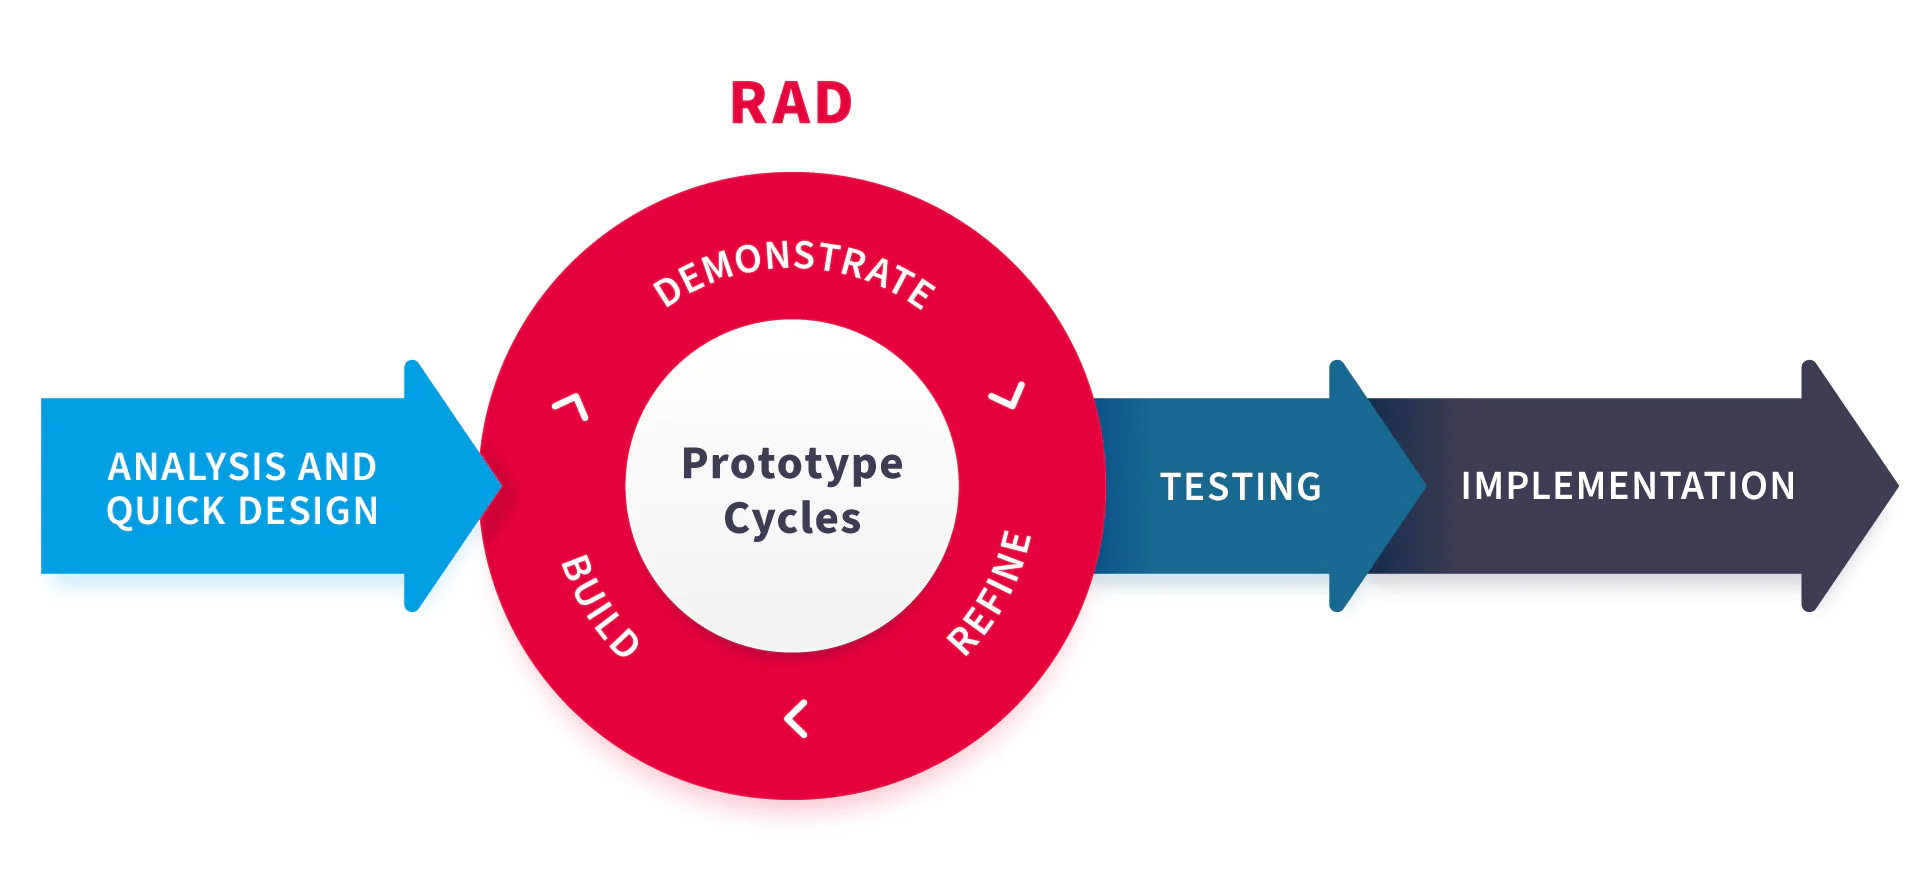
\includegraphics[width=1\linewidth]{figures/images/rad.png}
    \caption{Rapid Application Development (RAD) Model.}
    \label{fig:rad}
\end{figure}
    
\section{System Analysis}
The system analysis phase of the HRIS application development involves utilizing various methods to understand and define the system's functional and data requirements. These include information gathering, analytical methods, personnel consultation assessments, and content analysis. These methods aid in identifying user needs, defining system functionalities, and establishing the database schema. 

Through the use of visual tools like use Swim-lane Diagram, Use case Diagrams, Entity Relational Diagrams, and Gantt charts, the system analysis phase enables a comprehensive understanding of the HRIS application's scope and requirements. By employing a systematic approach to system analysis, the development team can ensure that the HRIS application is designed and implemented in alignment with the project objectives and user expectations.

    \subsection{Swim-lane Diagram}
    The Swim-lane diagram illustrates the process flow of the HRIS. The process begins when the user enters their login credentials. These credentials are unique to each University faculty employee, distinguishing them from other users in the system. Each user has different privileges and assignments set initially to access the system. After entering the credentials, the system validates them, granting the user access to the system. Once the user successfully logs in, they are directed to the dashboard where they can perform different actions depending on their privileges e.g., perform employee actions or tasks and HR overall general management.

    The identified roles i.e., Director, Sys. Admin, Attendance Monitoring and Checker, Training \& Dev. Specialist, Records Mgt. Specialist, Comp. \& Benefits Officer, ISS Officer, Recruitment \& Admin Staff, and Capability Bldg. Officer, are assigned specific tasks and responsibilities within the system. These responsibilities and privileges are outlined in table \ref*{tab:hris-basic-modules}. 

    \begin{figure}[H]
        \centering
        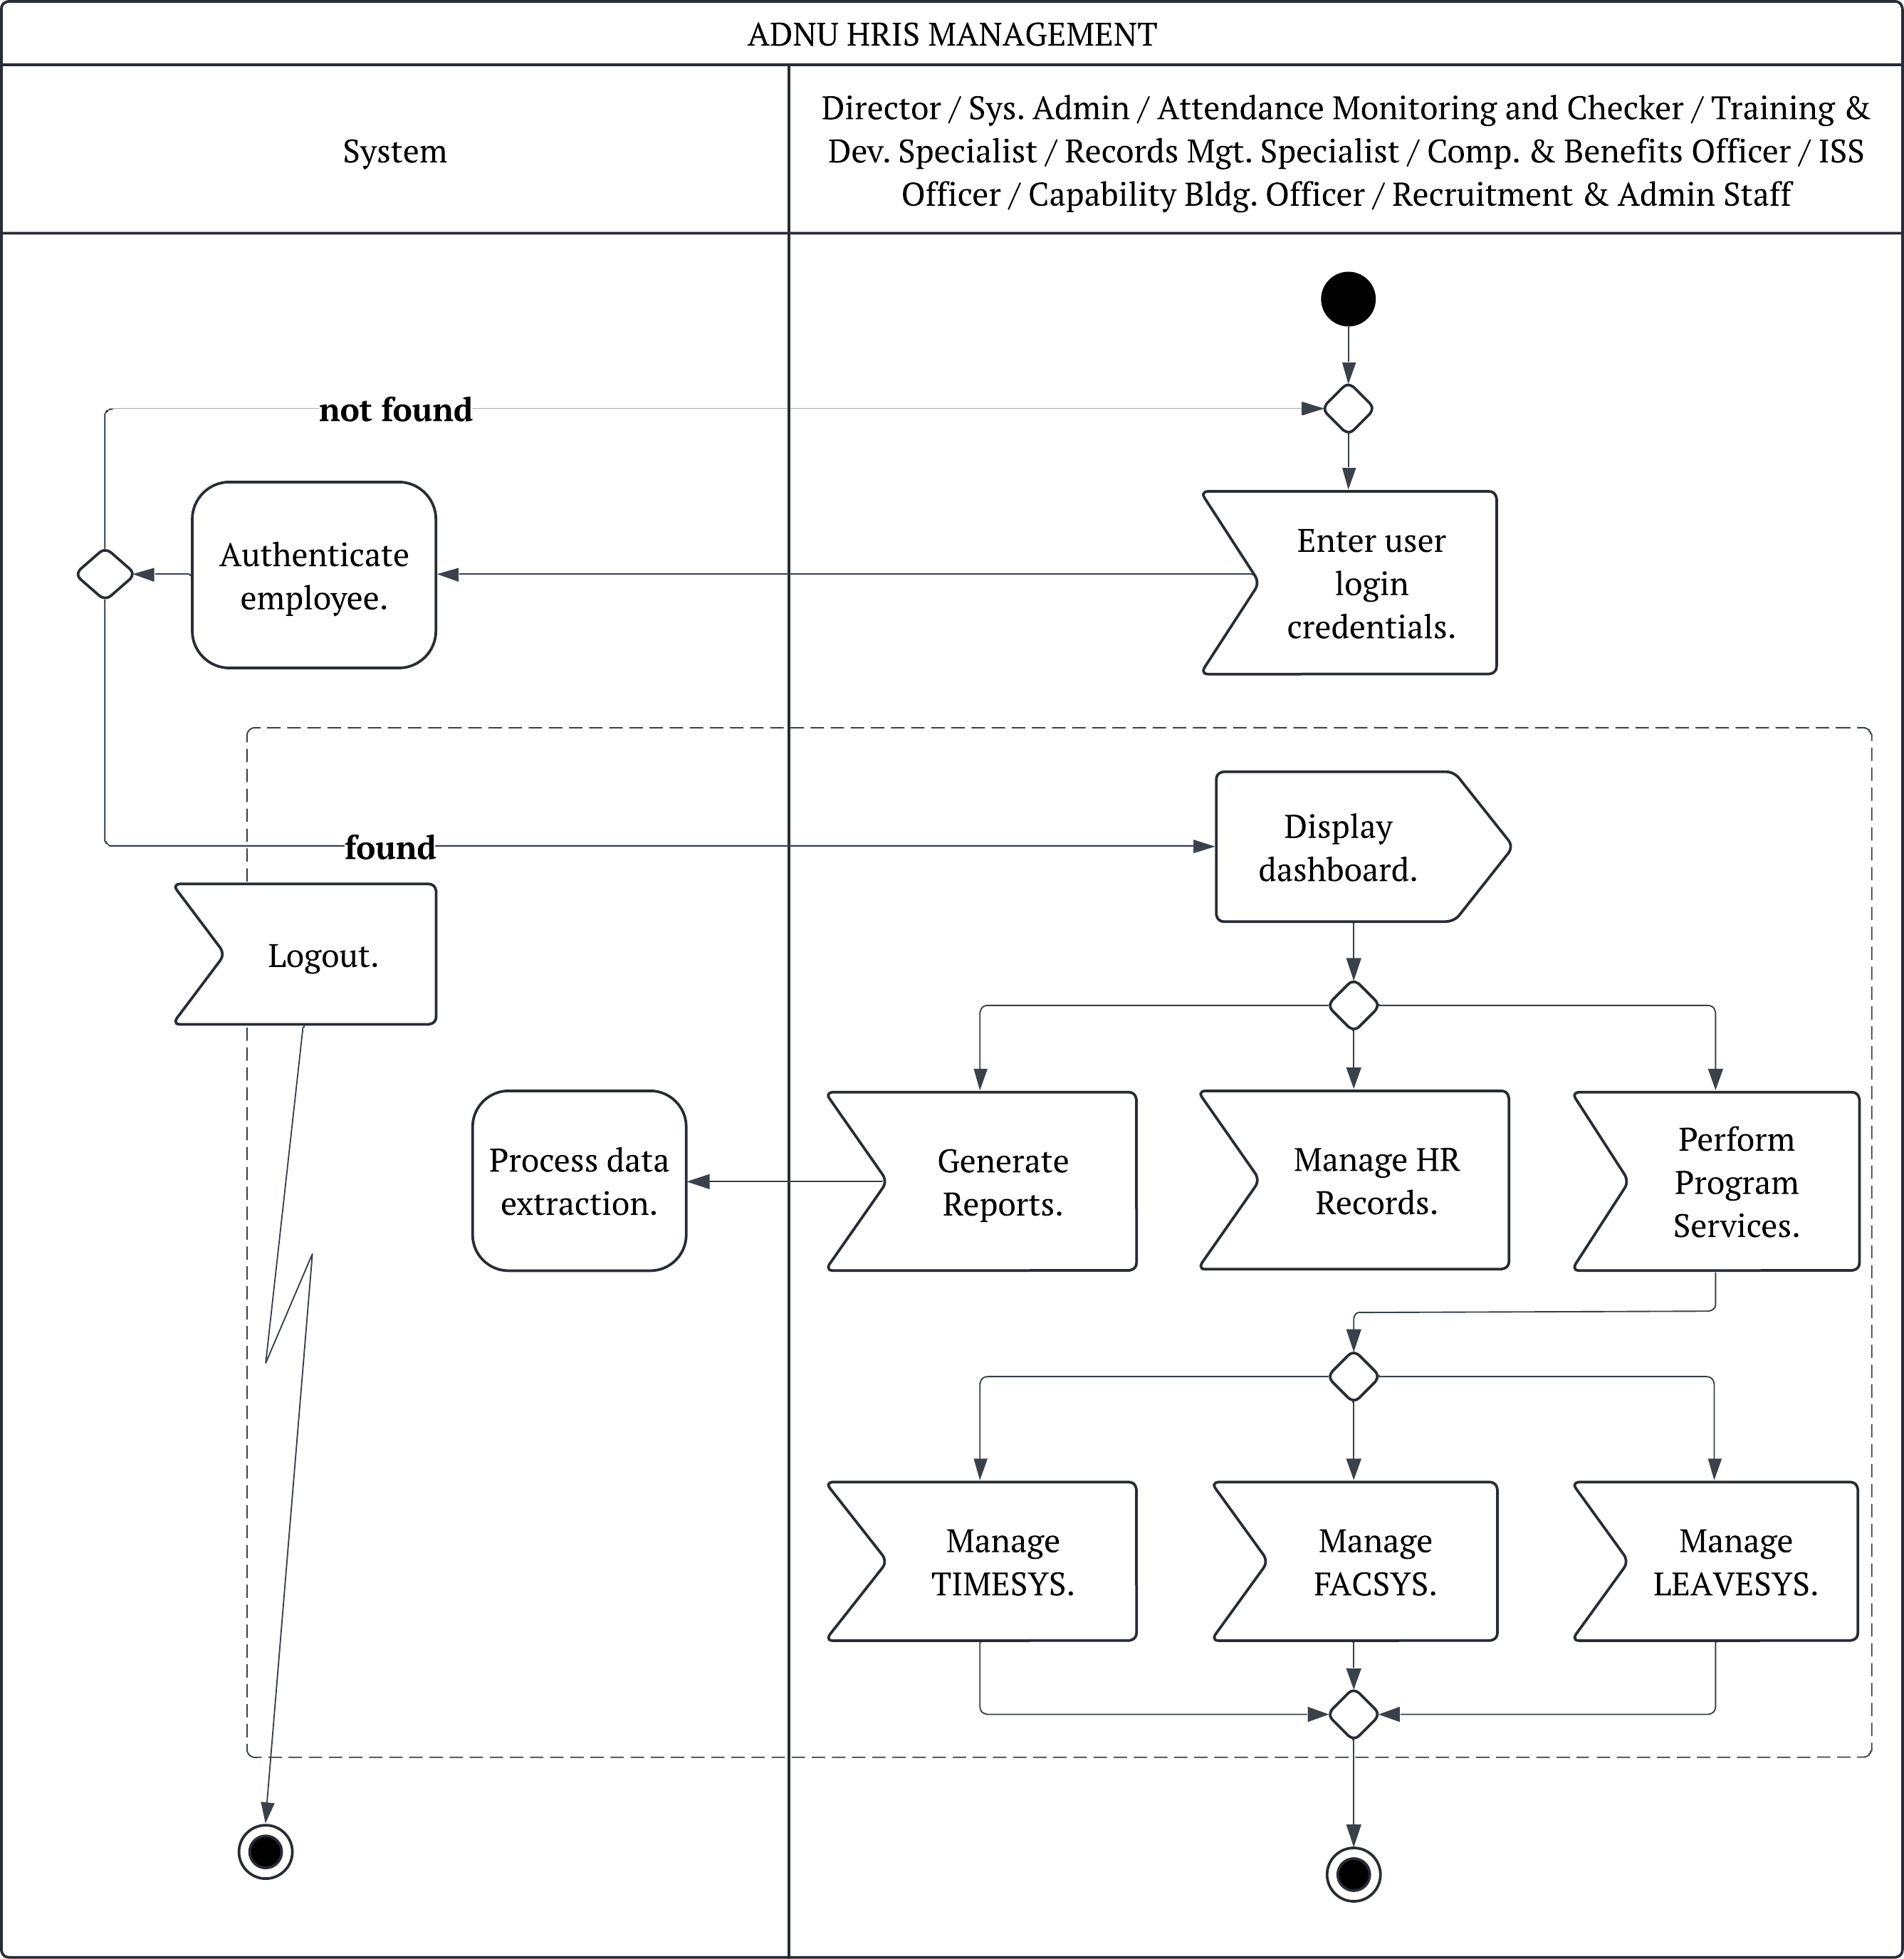
\includegraphics[width=1\linewidth]{figures/images/swimlane-admins.png}
        \caption{HRIS Swim-lane Diagram Model for HR Management.}
        \label{fig:swimlane-admins}
    \end{figure}

    Each roles area can perform admin privileges and manage different modules within the system. For these actions, they are processed and managed under the system to provide a streamlined operation for any users in the system. Higher admins will have access to core modules e.g., Manage employee/personnel containing the employee contacts, personal information, profiles, assignments, assignment archive, faculty rank, academic, academic awards, professional license, training attendance, Certificate of Employment (COE), and health record.

    Besides this, these admins can also generate different kinds of reports within the system e.g., performing data extraction, queries, employee performance evaluation, COE reports, contracts/appointment generation, etc.

    \begin{figure}[H]
        \centering
        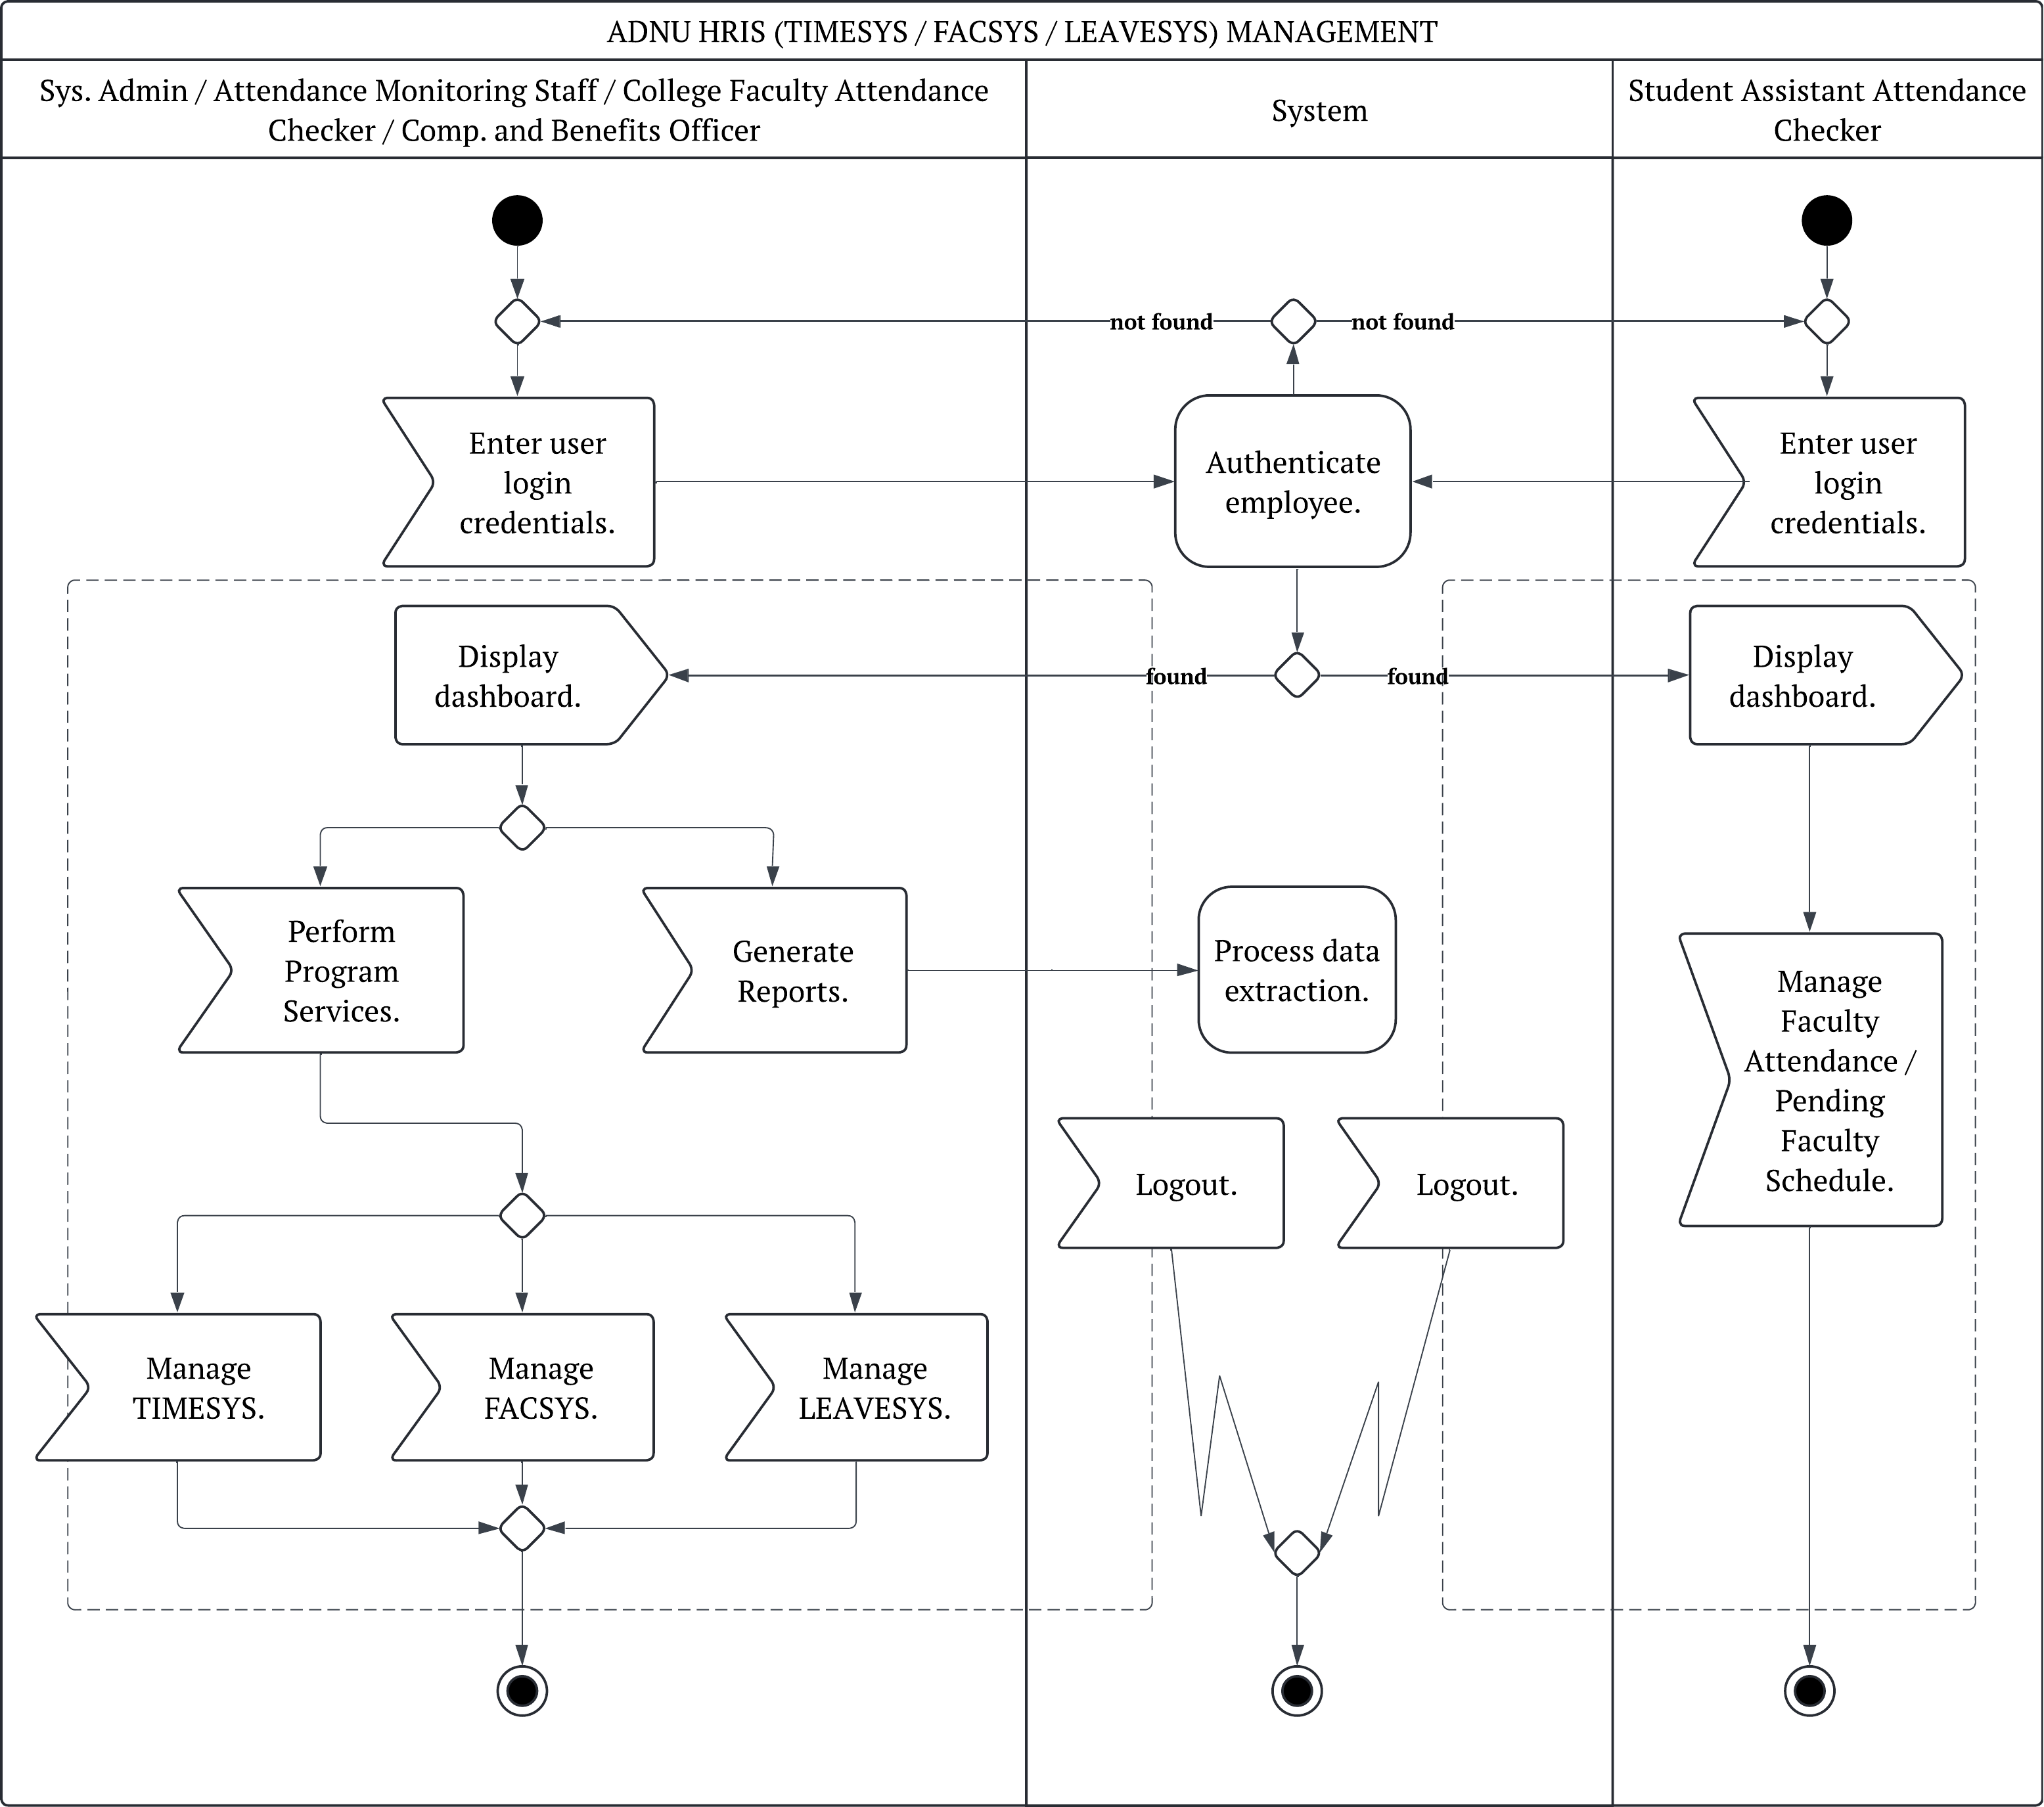
\includegraphics[width=1\linewidth]{figures/images/swimlane-sys-mgt.png}
        \caption{HRIS Swim-lane Diagram Model for TIMESYS, FACSYS, and LEAVESYS Management.}
        \label{fig:swimlane-sys-mgt}
    \end{figure}

    The system also includes modules for TIMESYS, FACSYS, and LEAVESYS. These modules are designed to manage employee attendance, faculty attendance, and employee leave applications, respectively. In the diagram, the identified roles along with their privilege are assigned to manage the three (3) SYS as well as allowing them to generate reports. Meanwhile, the Student Assistant Attendance Checker have lesser privilege and is assigned only to managing faculty attendance, faculty schedule, and managing pending faculty schedules.

    \subsection{Use Case Diagram}
    
    The use case diagram serves as a visual representation of the functional requirements of the system from an external user's perspective. It illustrates the interactions between users and the system, showcasing the various use cases and how they relate to each other. In the context of the HRIS application, the use case diagram will outline the different functionalities that users can perform within the system, such as employee management, payroll processing, and performance evaluation. By mapping out these interactions, the use case diagram helps in identifying the system's behavior and the roles of different users in the HRIS application.

    \begin{figure}[H]
        \centering
        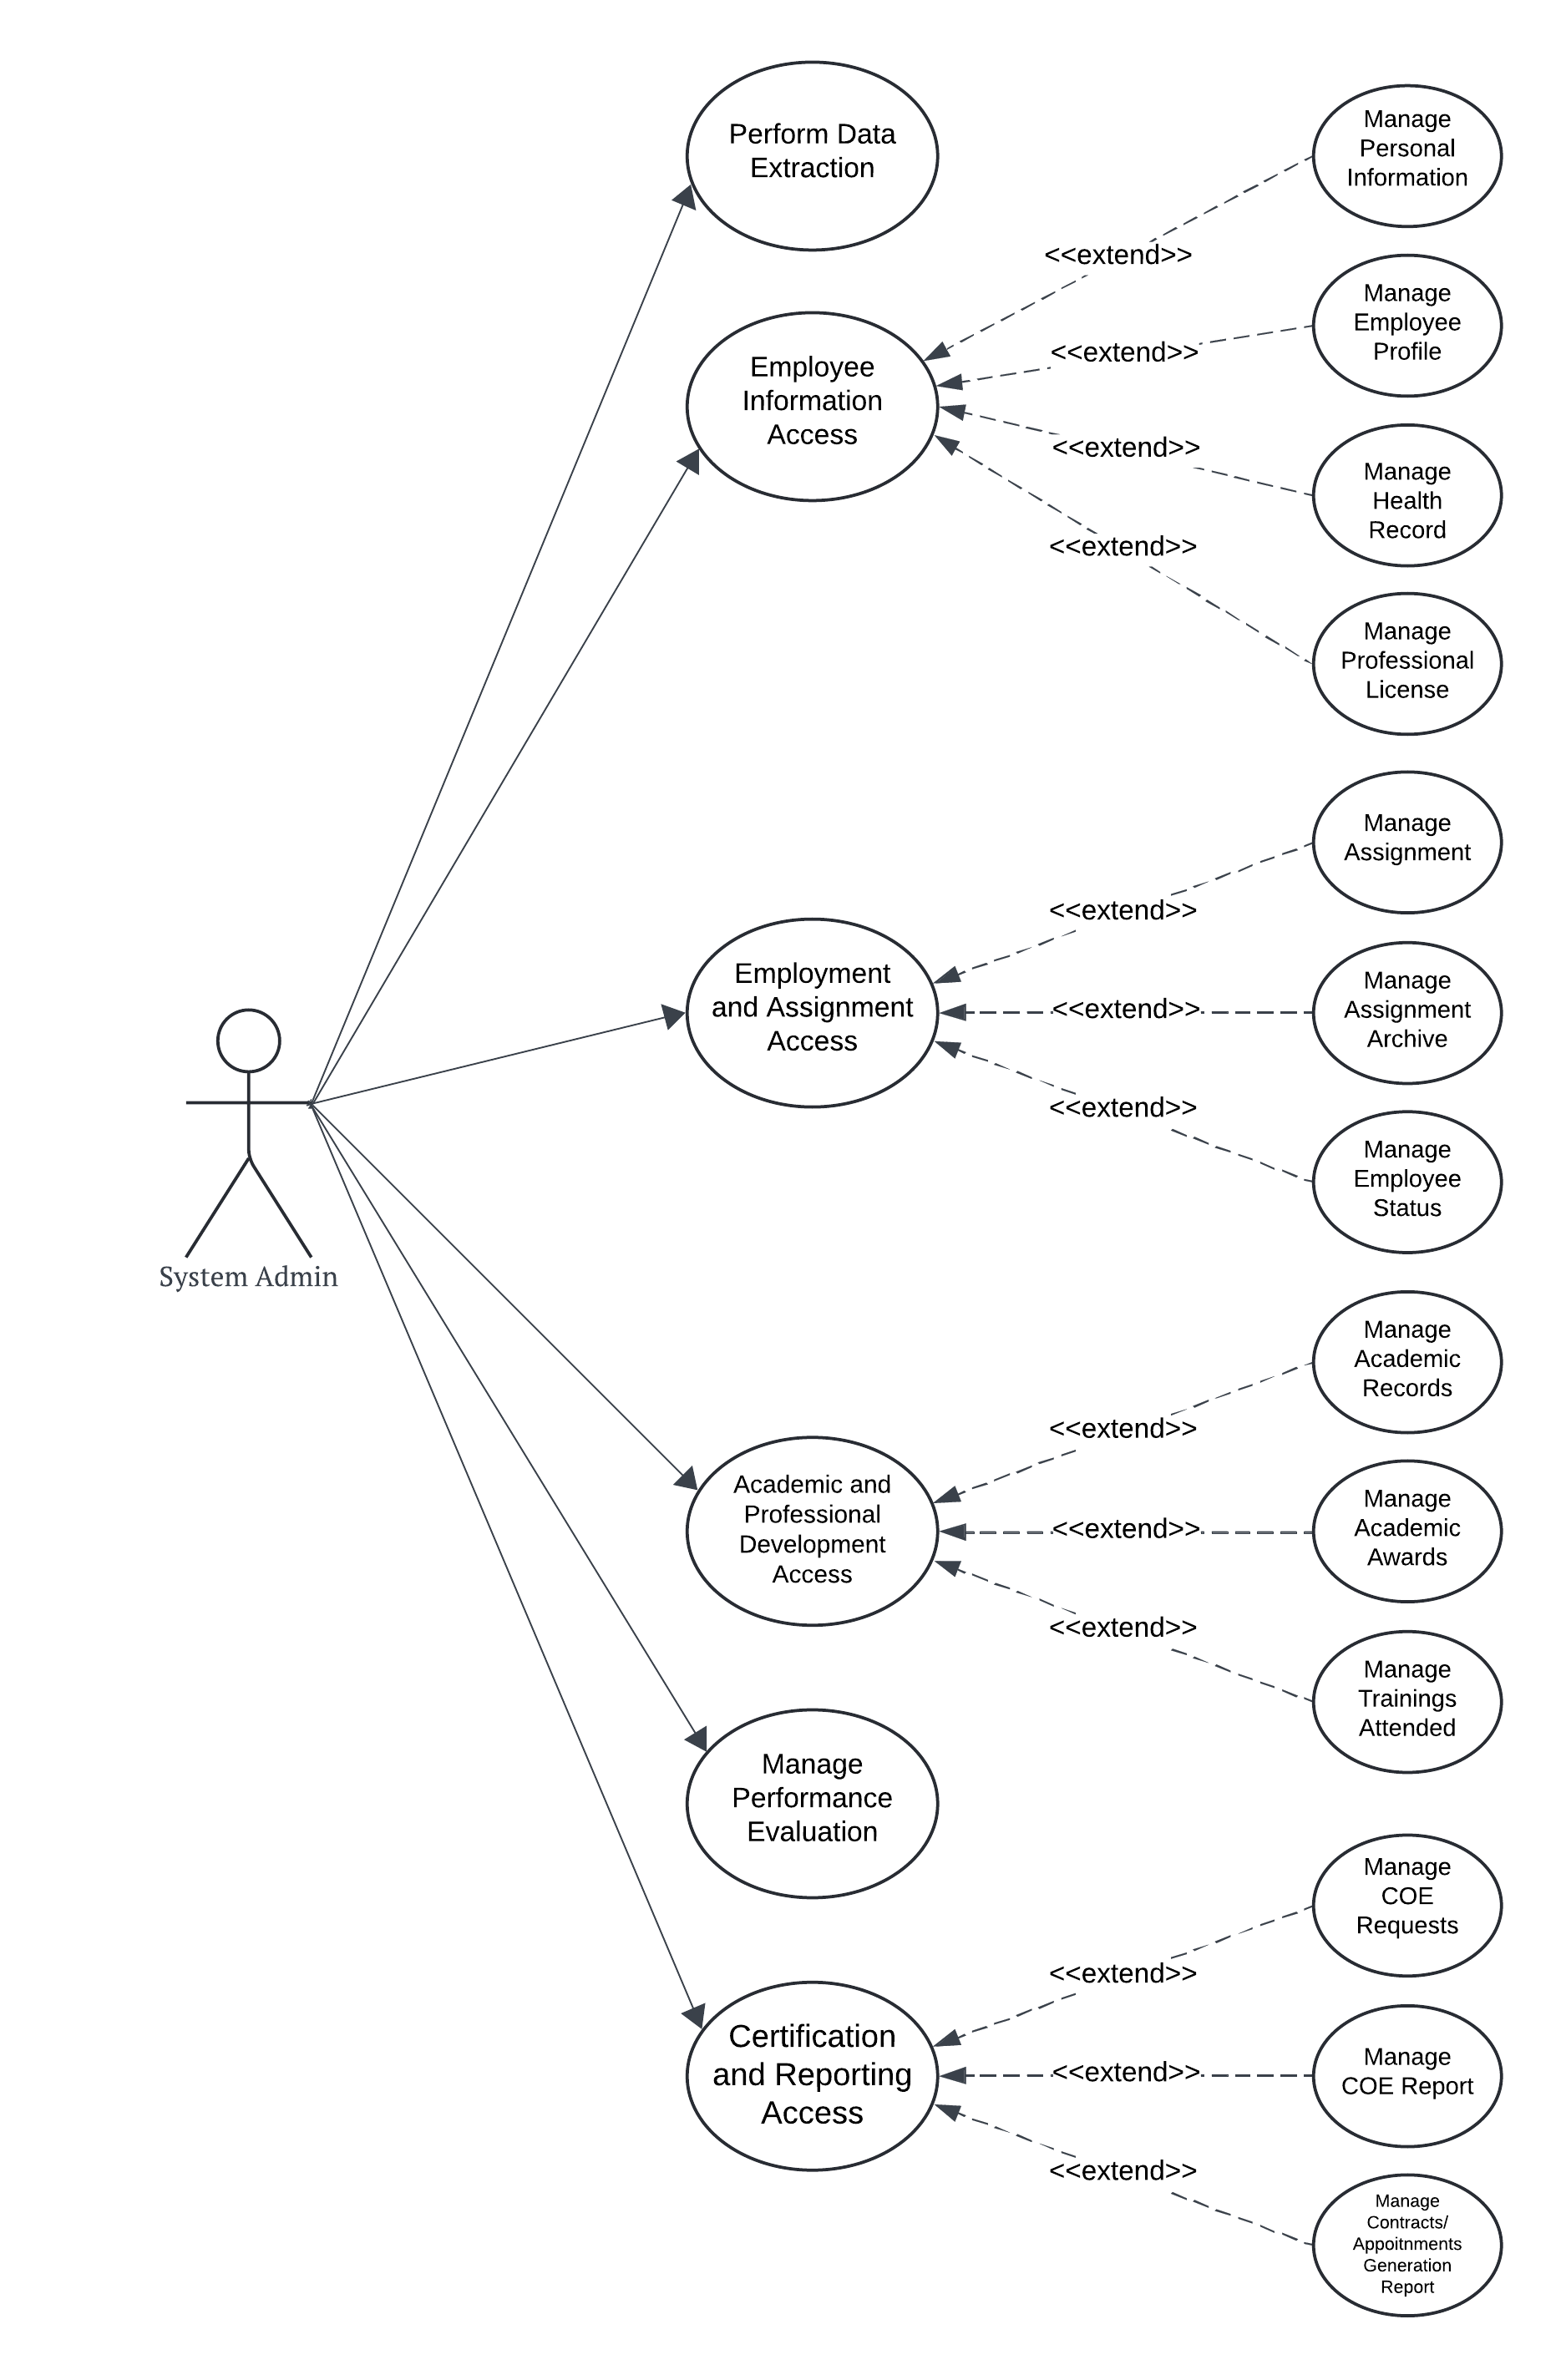
\includegraphics[width=0.9\linewidth]{figures/images/use-case-basic-1.png}
        \caption{HRIS Basic Modules Use Case Diagram: System Admin.}
        \label{fig:use-case-basic-1}
    \end{figure}

    \begin{figure}[H]
        \centering
        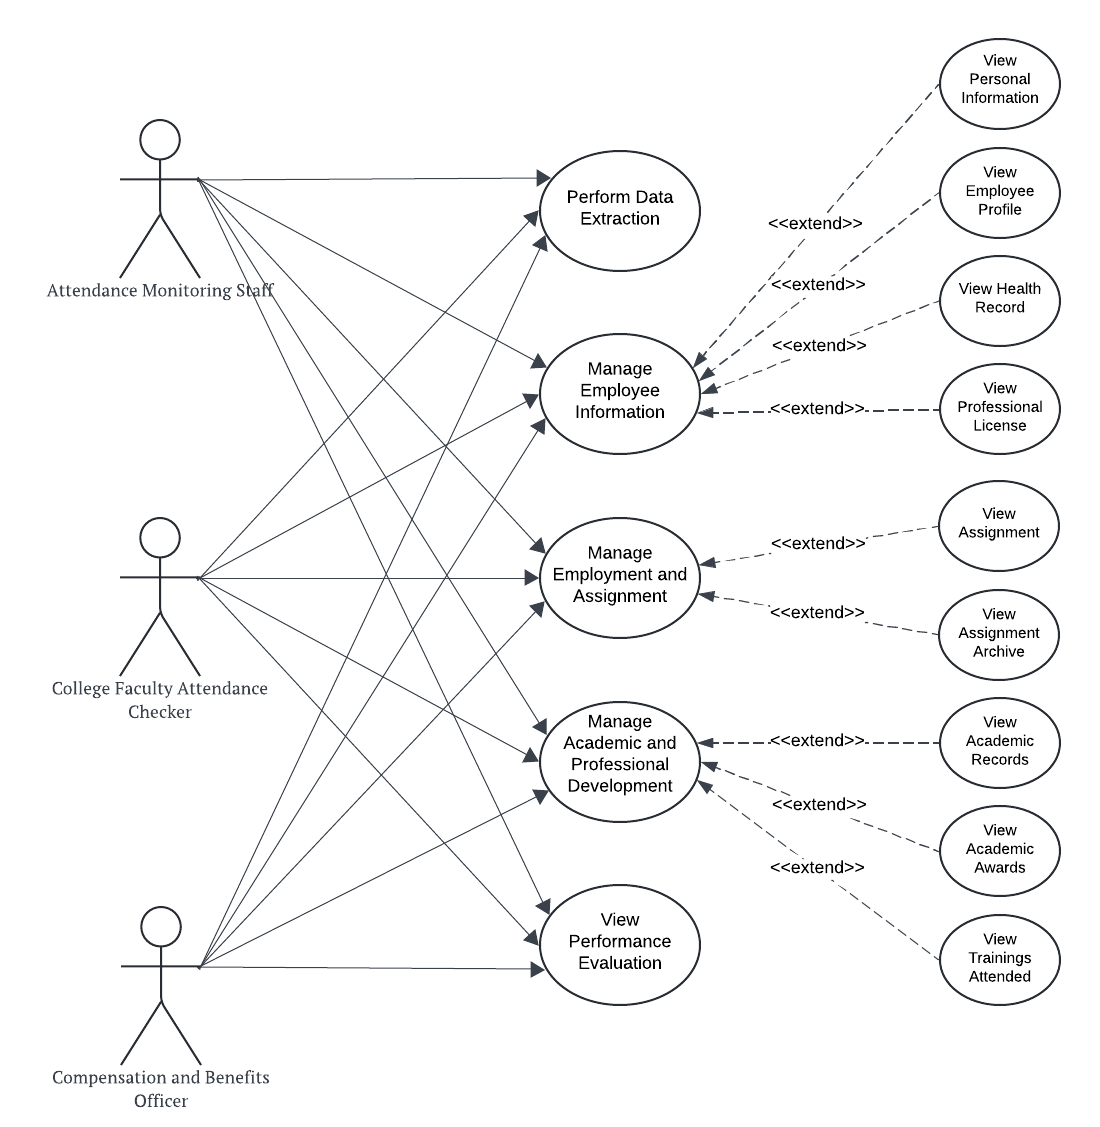
\includegraphics[width=0.9\linewidth]{figures/images/use-case-basic-2.png}
        \caption{HRIS Basic Modules Use Case Diagram: Attendance Monitoring Staff, College Faculty Attendance Checker, and Compensation and Benefits Officer.}
        \label{fig:use-case-basic-2}
    \end{figure}

    \begin{figure}[H]
        \centering
        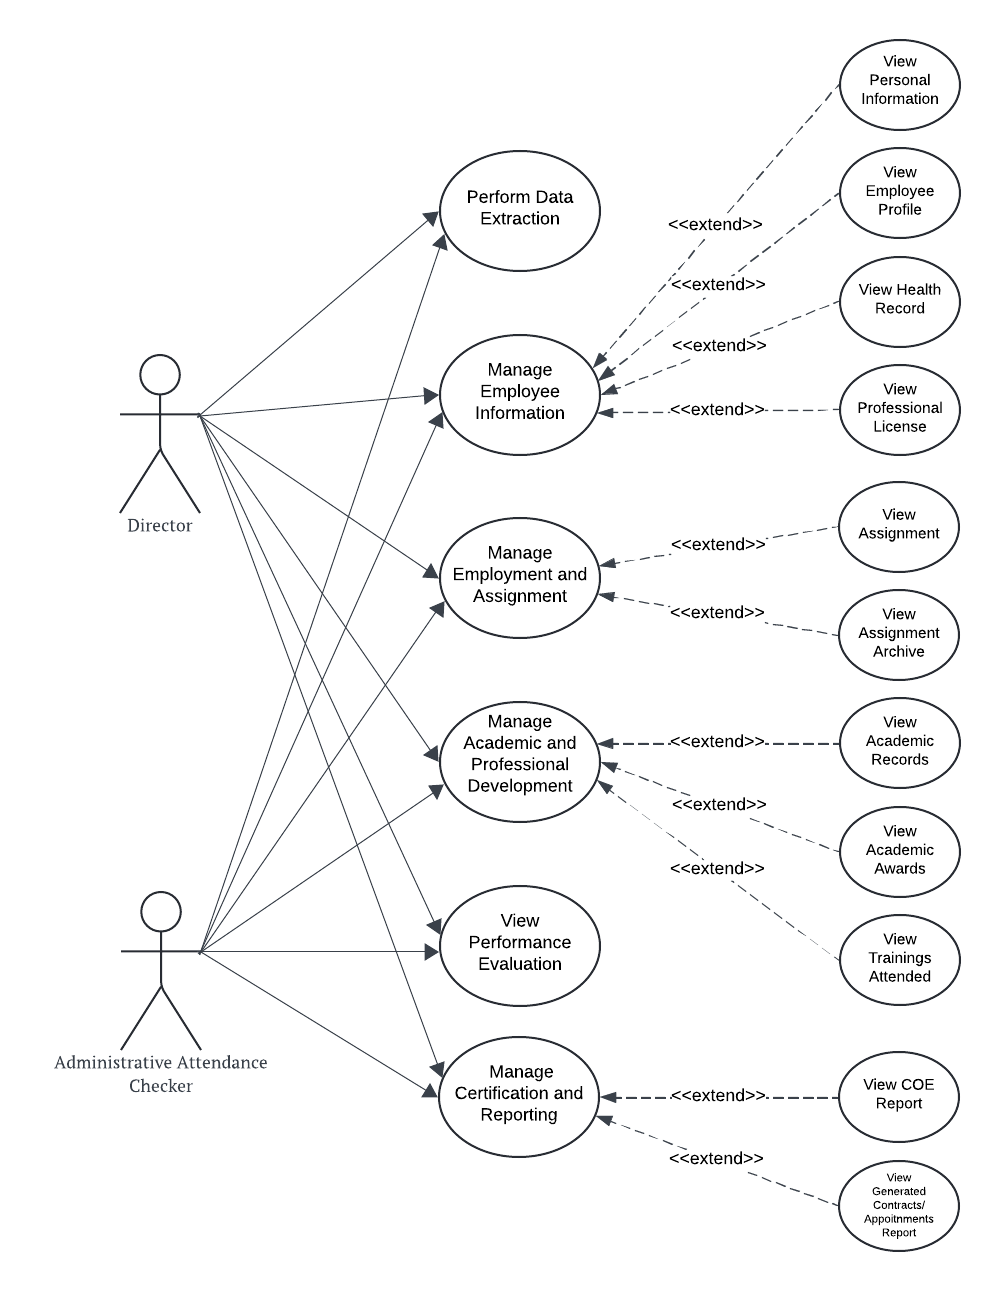
\includegraphics[width=0.9\linewidth]{figures/images/use-case-basic-3.png}
        \caption{HRIS Basic Modules Use Case Diagram: Director and Administrative Assistant.}
        \label{fig:use-case-basic-3}
    \end{figure}

    \begin{figure}[H]
        \centering
        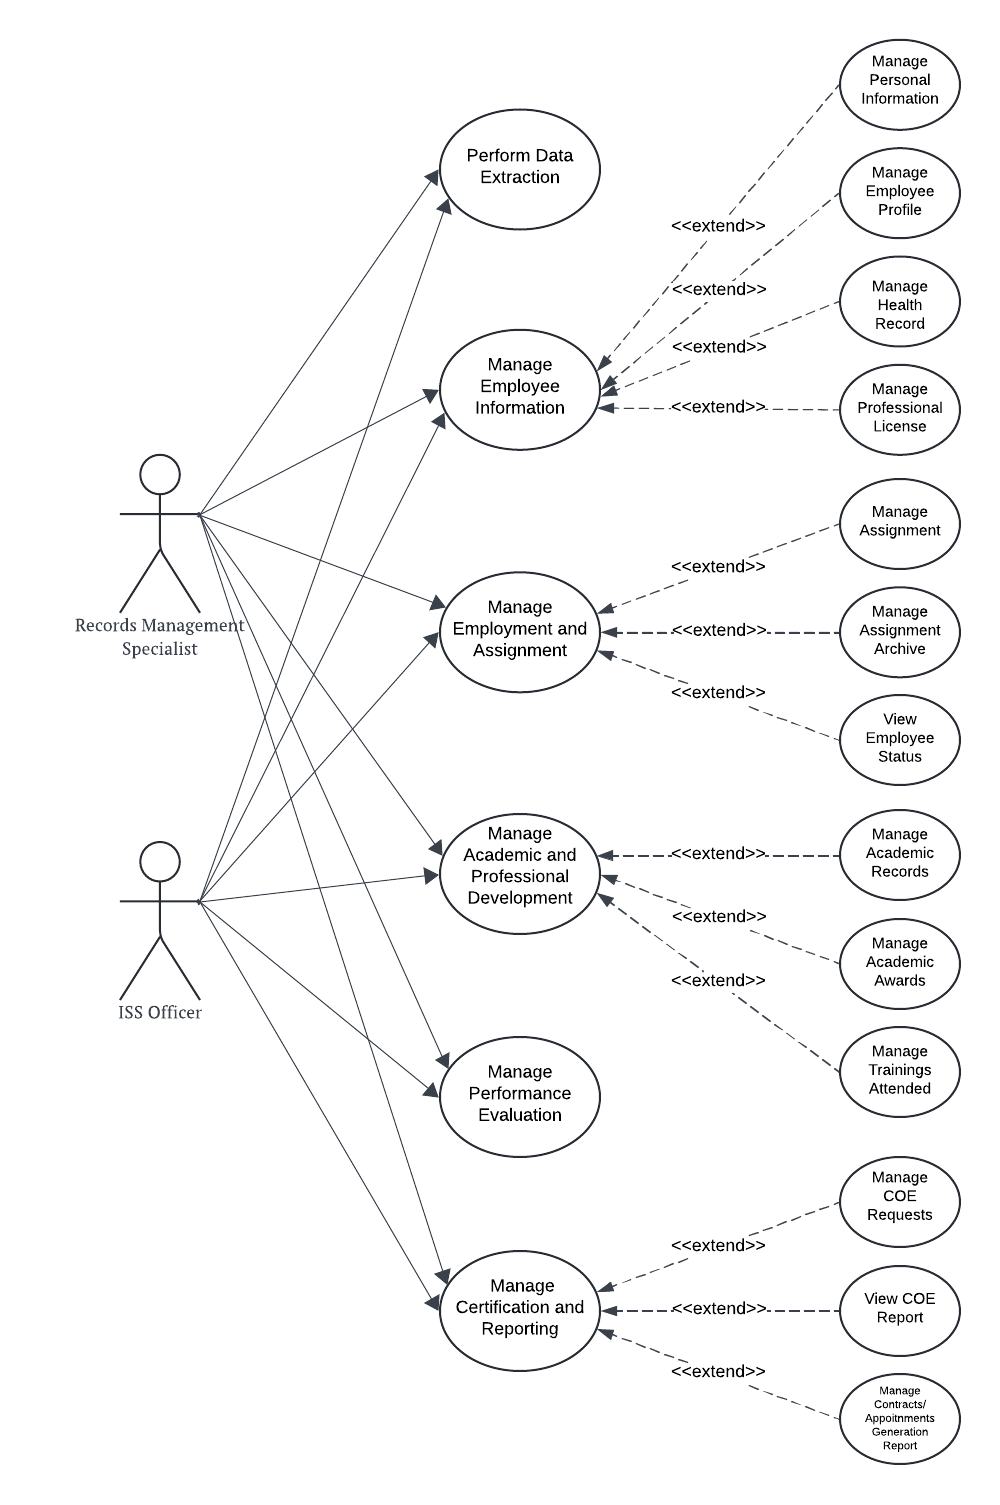
\includegraphics[width=0.9\linewidth]{figures/images/use-case-basic-4.png}
        \caption{HRIS Basic Modules Use Case Diagram: Records Management Specialist and ISS Officer.}
        \label{fig:use-case-basic-4}
    \end{figure}

    \begin{figure}[H]
        \centering
        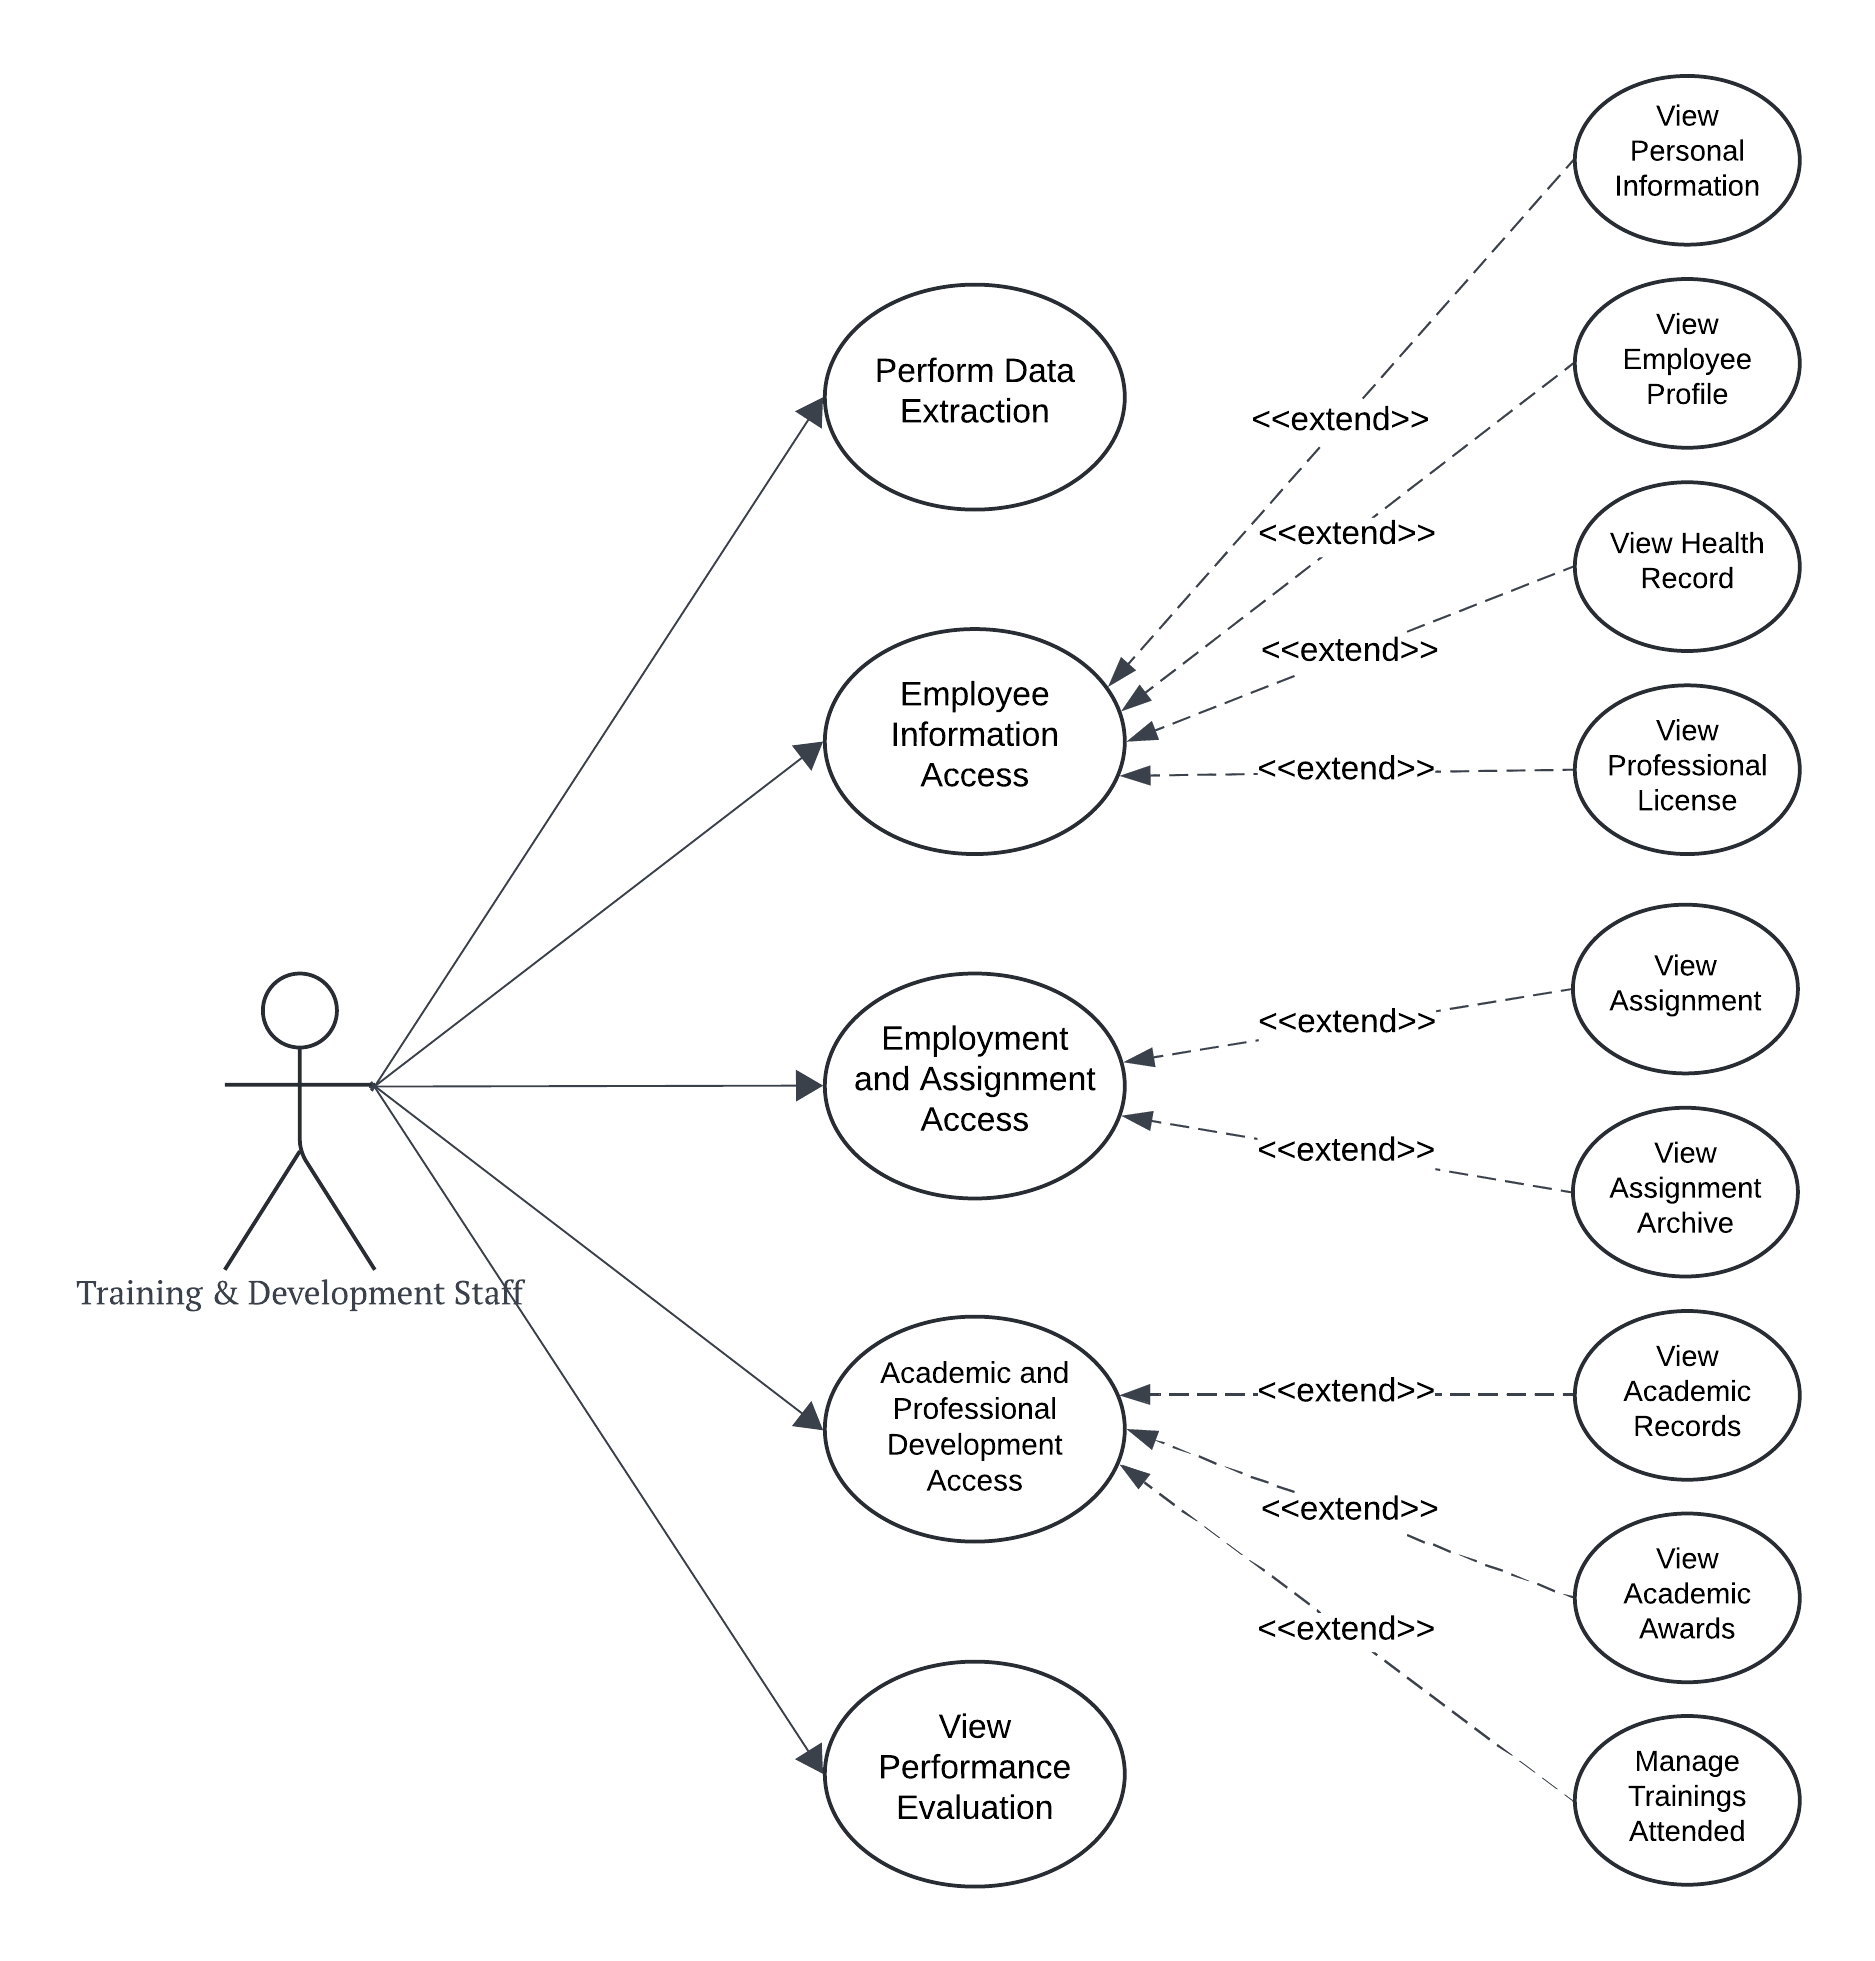
\includegraphics[width=0.9\linewidth]{figures/images/use-case-basic-5.png}
        \caption{HRIS Basic Modules Use Case Diagram: Training and Development Staff.}
        \label{fig:use-case-basic-5}
    \end{figure}

    \begin{figure}[H]
        \centering
        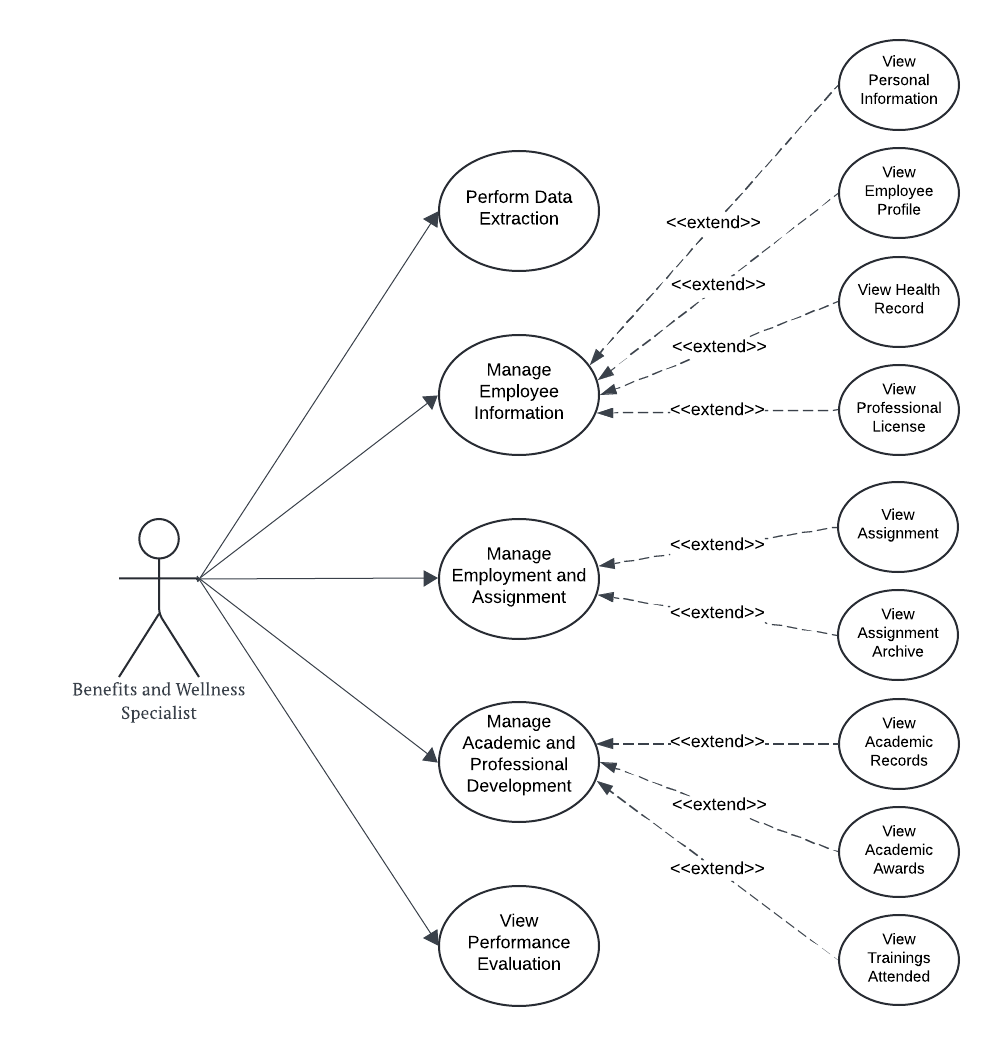
\includegraphics[width=0.9\linewidth]{figures/images/use-case-basic-6.png}
        \caption{HRIS Basic Modules Use Case Diagram: Benefits and Wellness Specialist.}
        \label{fig:use-case-basic-6}
    \end{figure}

    \begin{figure}[H]
        \centering
        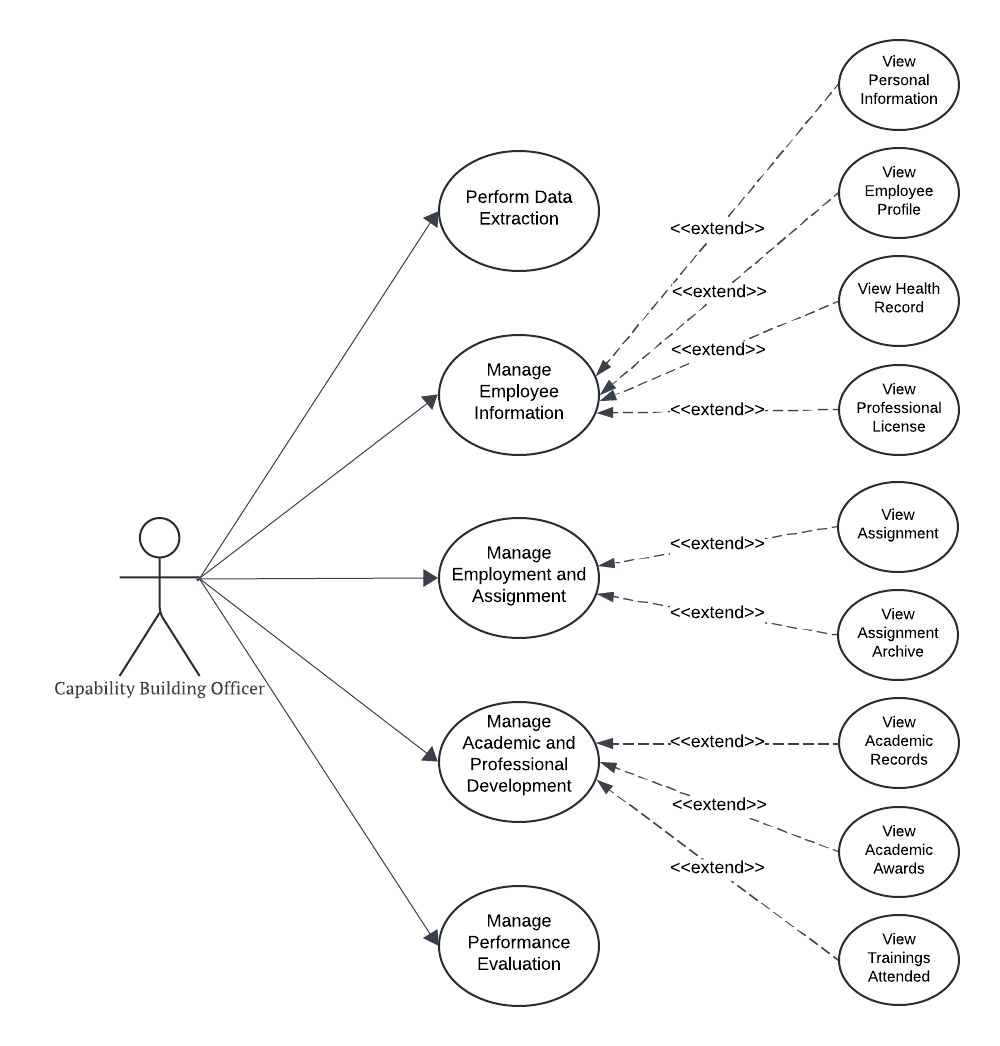
\includegraphics[width=0.9\linewidth]{figures/images/use-case-basic-7.png}
        \caption{HRIS Basic Modules Use Case Diagram: Capability Building Officer.}
        \label{fig:use-case-basic-7}
    \end{figure}

    \begin{figure}[H]
        \centering
        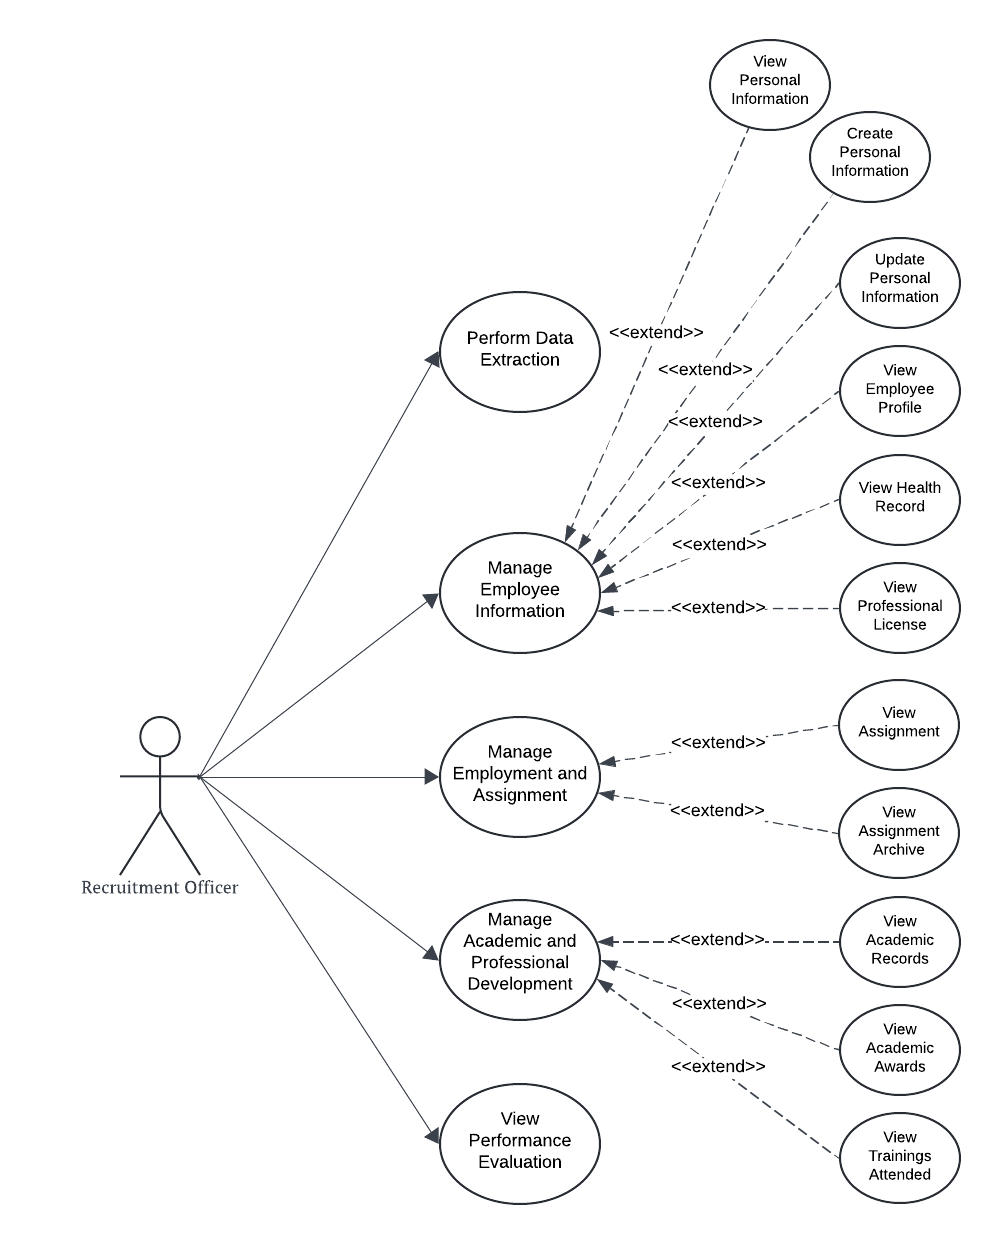
\includegraphics[width=0.9\linewidth]{figures/images/use-case-basic-8.png}
        \caption{HRIS Basic Modules Use Case Diagram: Recruitment Officer.}
        \label{fig:use-case-basic-8}
    \end{figure}

    \begin{figure}[H]
        \centering
        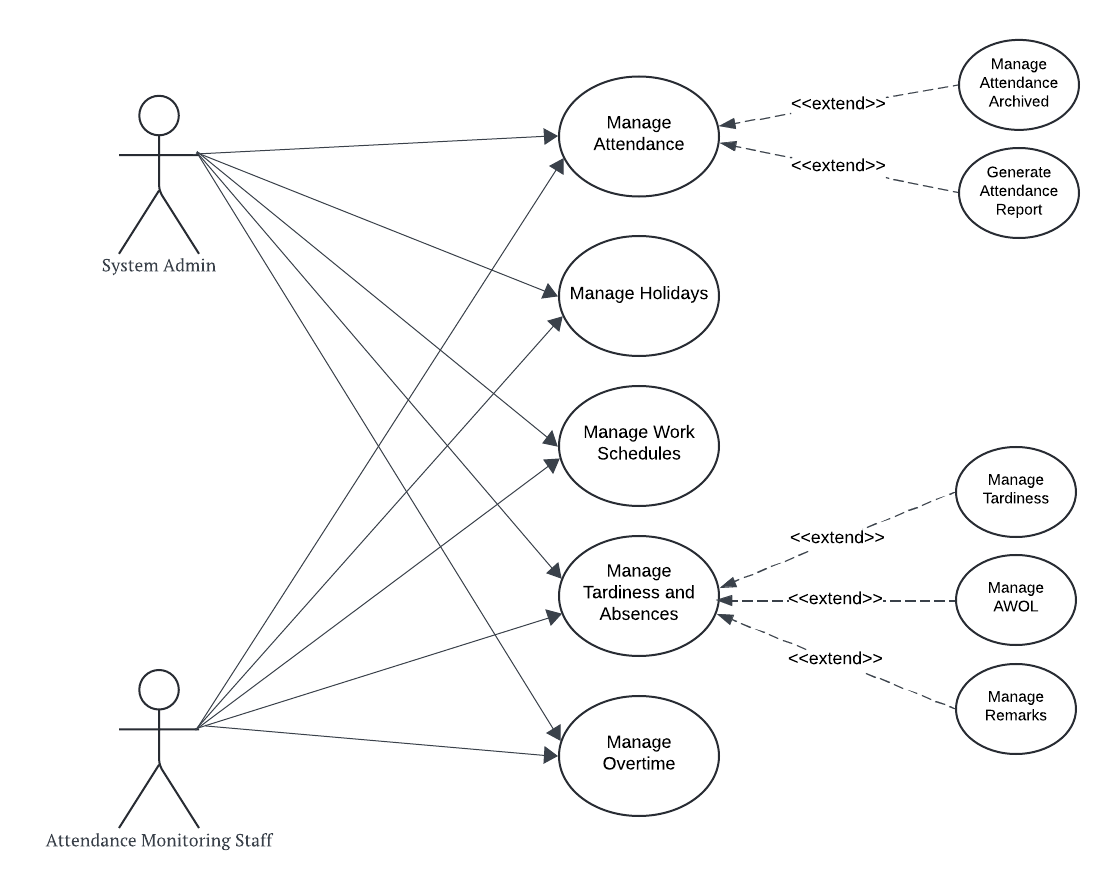
\includegraphics[width=0.9\linewidth]{figures/images/use-case-time-1.png}
        \caption{HRIS TIMESYS Module: System Admin and Attendance Monitoring Staff.}
        \label{fig:use-case-time-1}
    \end{figure}

    \begin{figure}[H]
        \centering
        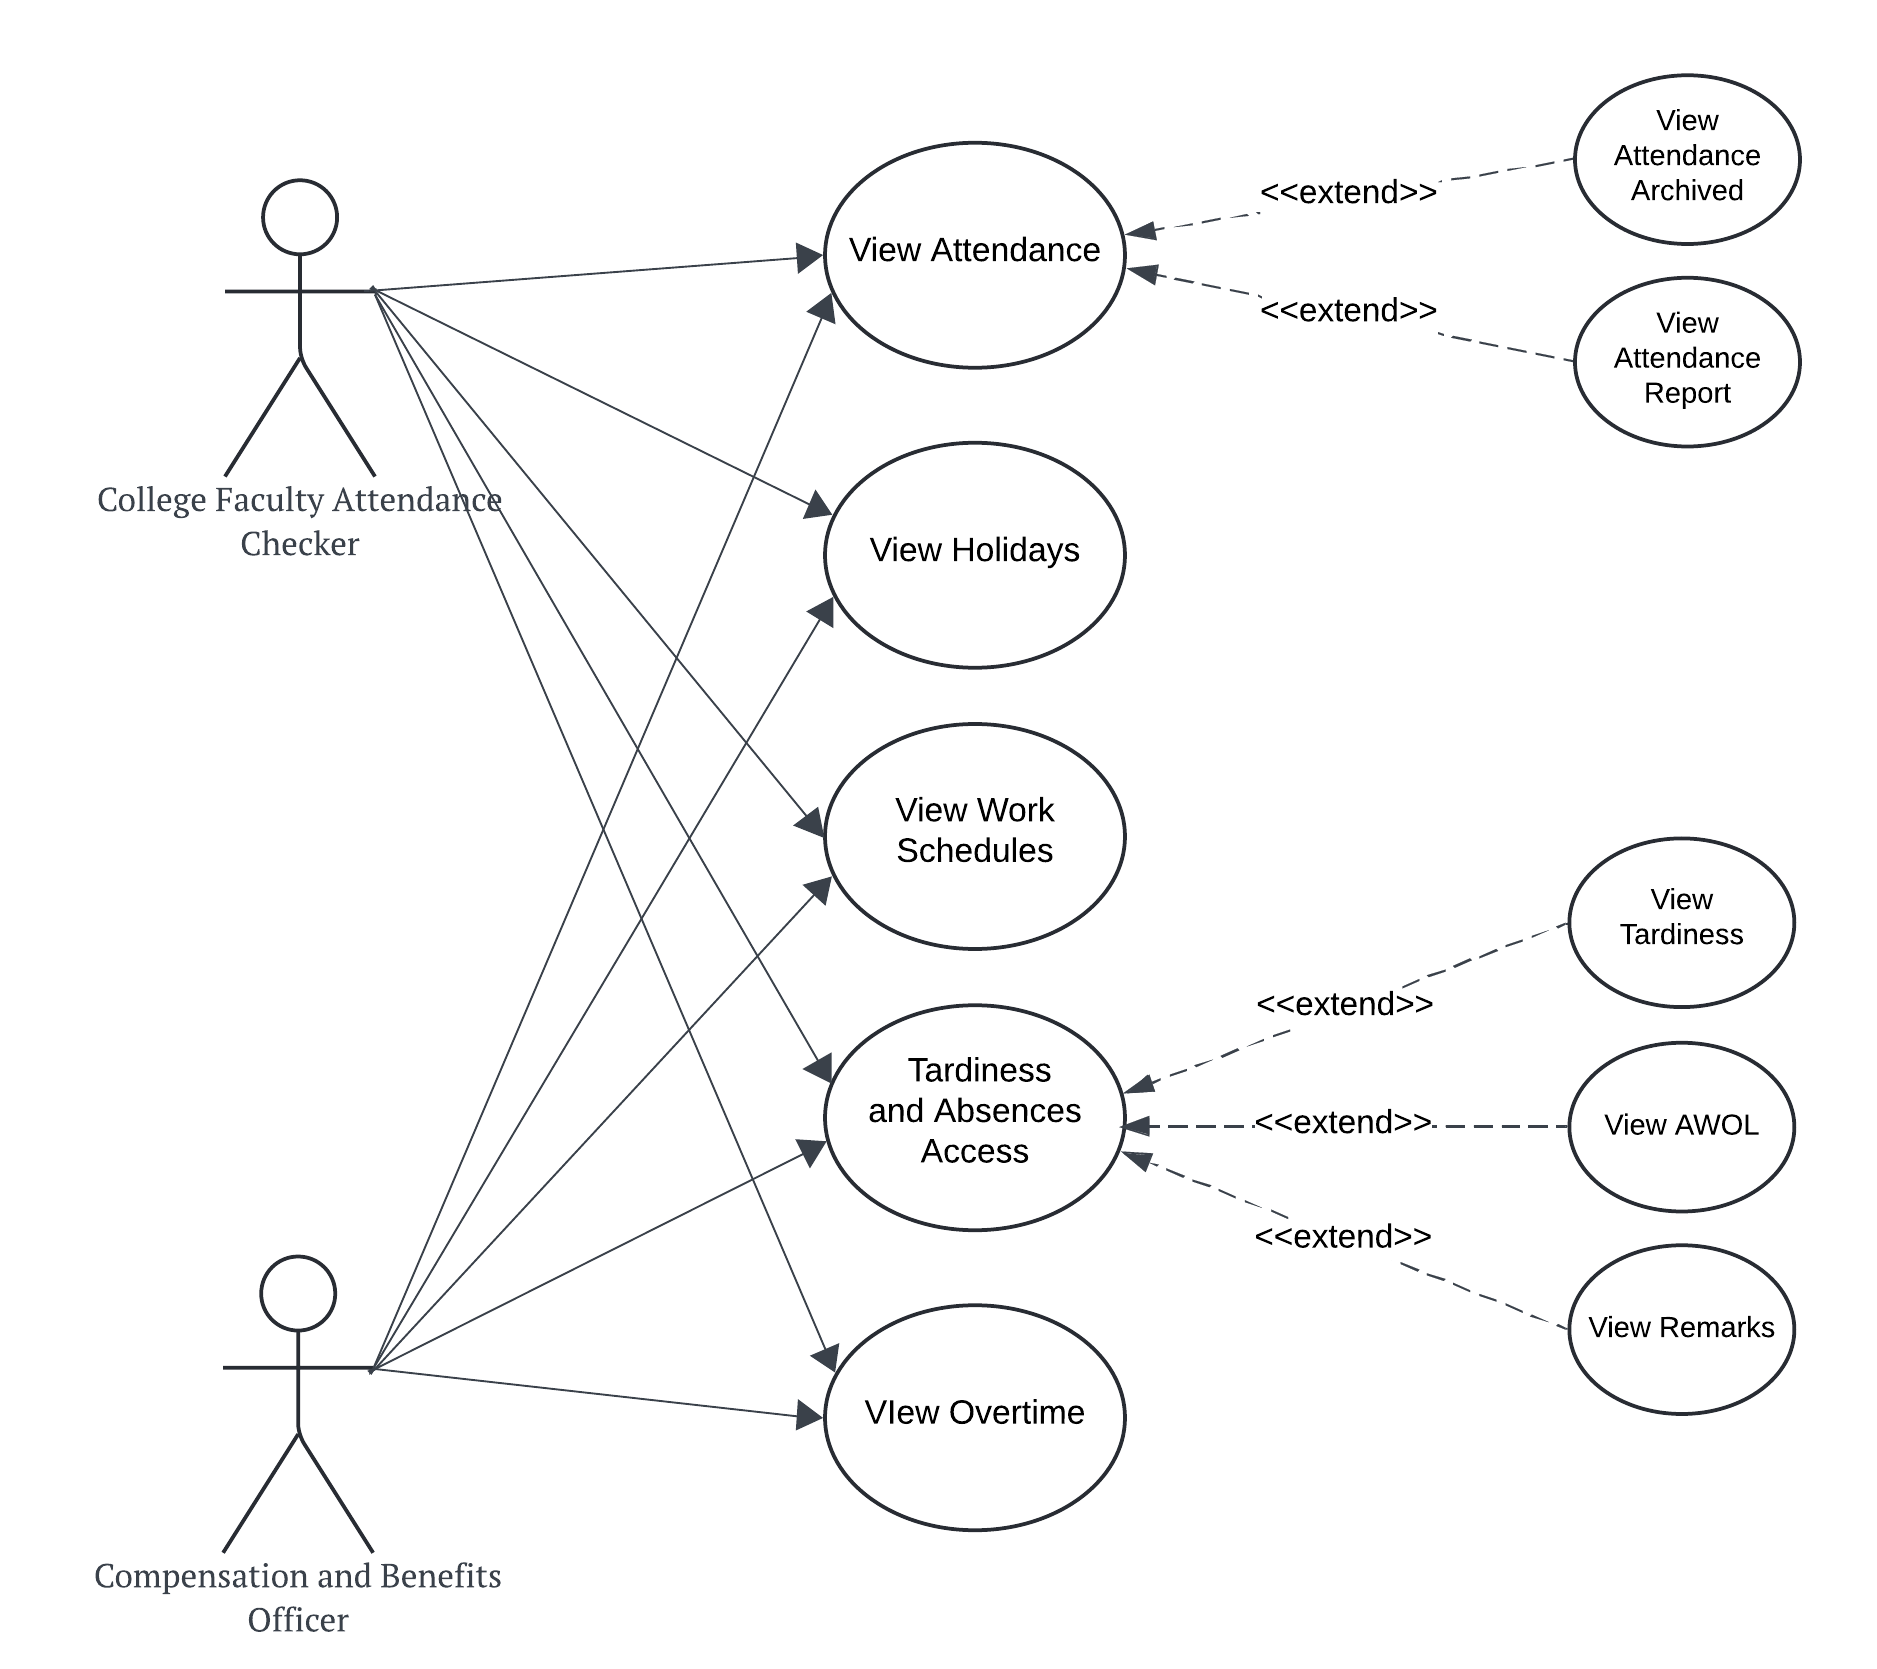
\includegraphics[width=0.9\linewidth]{figures/images/use-case-time-2.png}
        \caption{HRIS TIMESYS Module: College Faculty Attedance Checker and Compensation and Benefits Officer.}
        \label{fig:use-case-time-2}
    \end{figure}

    \begin{figure}[H]
        \centering
        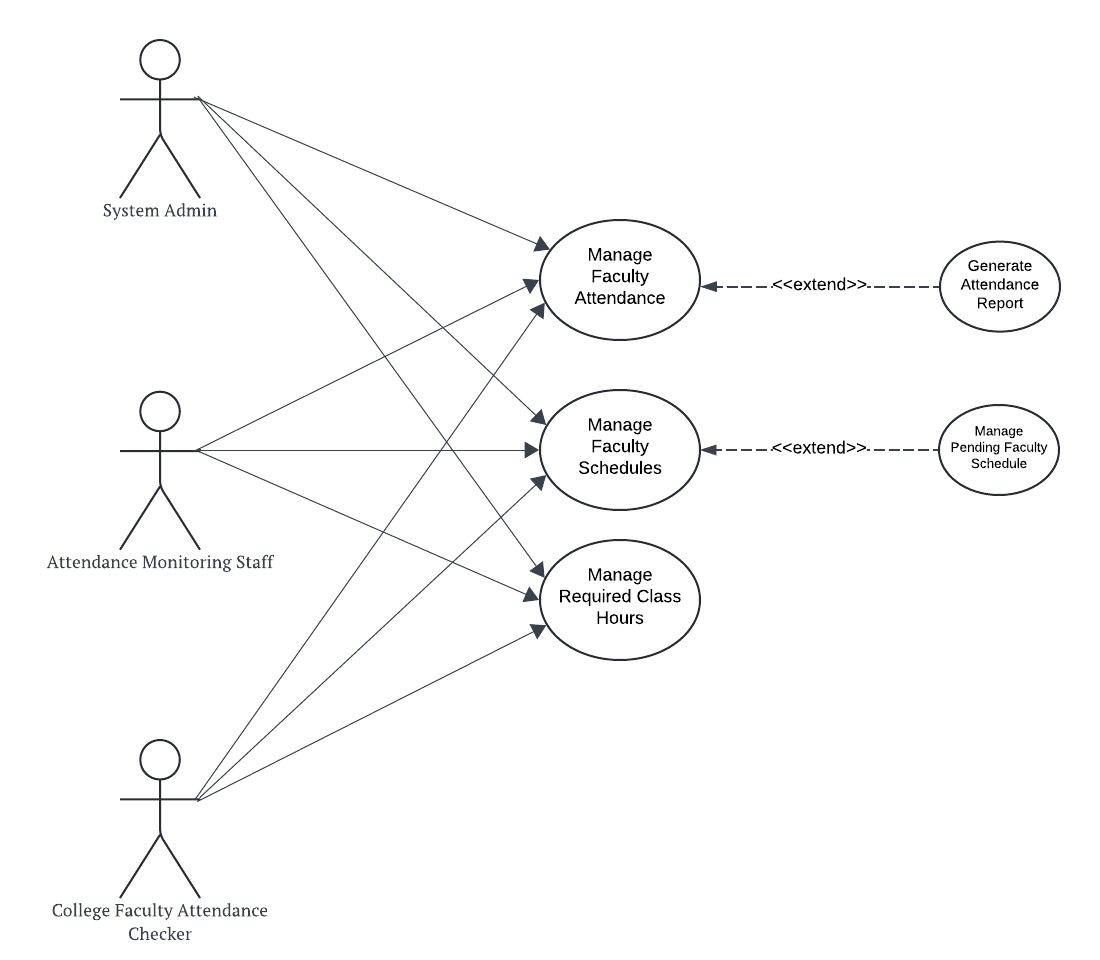
\includegraphics[width=0.9\linewidth]{figures/images/use-case-fac-1.png}
        \caption{HRIS FACSYS Module: System Admin, Attendance Monitoring Staff, and College Faculty Attendance Checker.}
        \label{fig:use-case-fac-1}
    \end{figure}

    \begin{figure}[H]
        \centering
        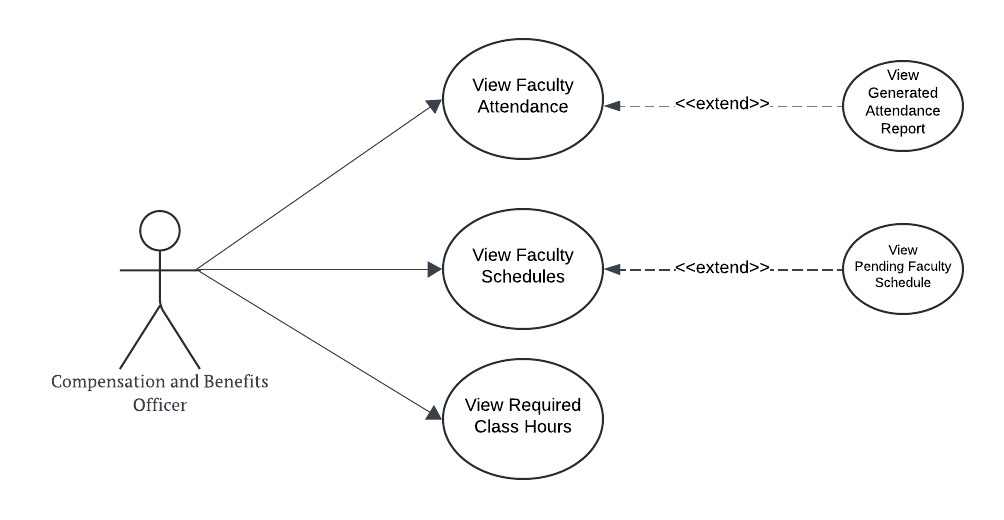
\includegraphics[width=0.9\linewidth]{figures/images/use-case-fac-2.png}
        \caption{HRIS FACSYS Module: Compensation and Benefits Officer.}
        \label{fig:use-case-fac-2}
    \end{figure}

    \begin{figure}[H]
        \centering
        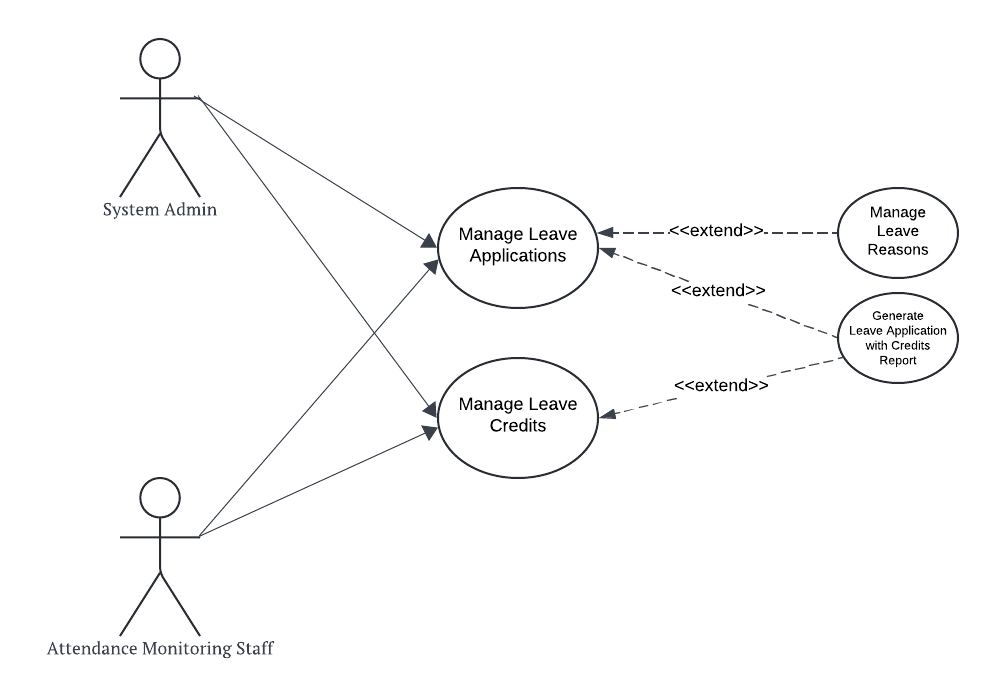
\includegraphics[width=0.9\linewidth]{figures/images/use-case-leave-1.png}
        \caption{HRIS LEAVESYS Module: System Admin and Attendance Monitoring Staff.}
        \label{fig:use-case-leave-1}
    \end{figure}

    \begin{figure}[H]
        \centering
        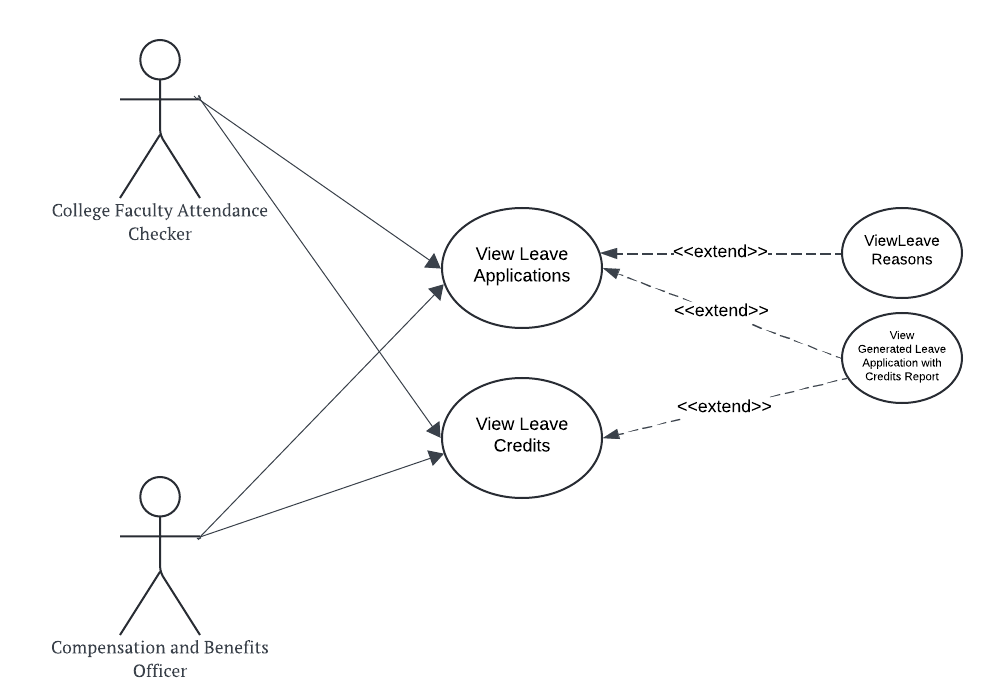
\includegraphics[width=0.9\linewidth]{figures/images/use-case-leave-2.png}
        \caption{HRIS LEAVESYS Module: College Faculty Attedance Checker and Compensation and Benefits Officer.}
        \label{fig:use-case-leave-2}
    \end{figure}



    
    
    \subsection{Entity Relational Diagram}
    
    The Entity Relational Diagram (ERD) will be used to visually represent the database structure that defines the relationships between different entities in the system and how they are related to one another through cardinalities and relationships. In the case of the HRIS application, MIS has provided ready access to the database scheme in preparation for the migration process. This ERD represents the various entities such as employees, departments, positions, and their relationships with each other. 
    
    Creating an ERD will allow the developers to design a database schema that accurately represents the data requirements of the HRIS system. This diagram is not only crucial for ensuring data integrity, normalization, and efficient data retrieval, but will also standardize and comply with the DBA requirements of the MIS for merge request and reviewing processes.

    \begin{figure}[H]
        \centering
        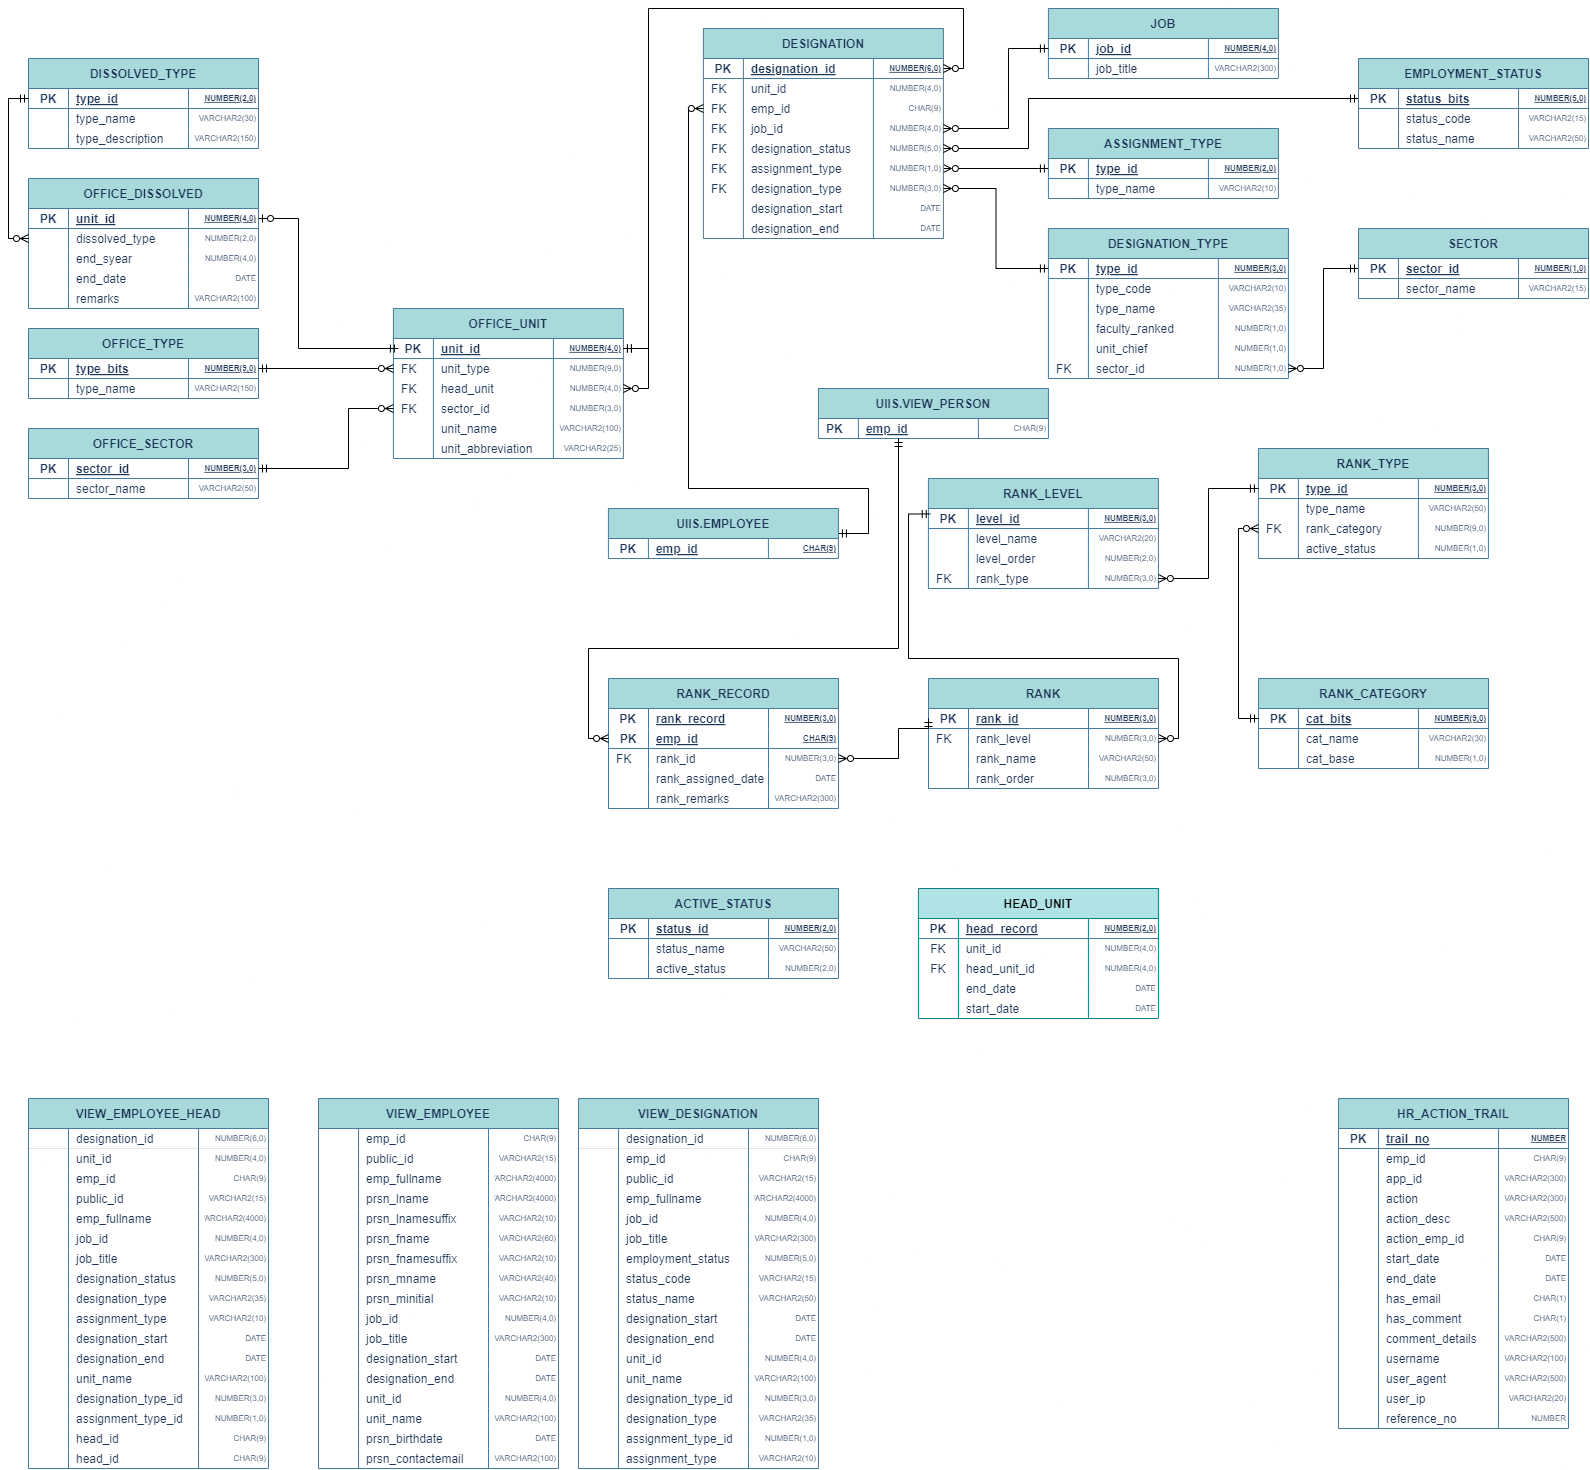
\includegraphics[width=1\linewidth]{figures/images/erd-hris.png}
        \caption{HRIS Core ERD Model.}
        \label{fig:erd-hris}
    \end{figure}

    This segment of the ERD model \ref*{fig:erd-hris} represents the core of HRIS, focusing on Employee Data Management. It includes tables such as EMPLOYMENT\_STATUS, JOB, OFFICE\_TYPE, OFFICE\_UNIT, and OFFICE\_SECTOR to categorize employment statuses, job details, and office structures. Additionally, it features a multi-tiered employee ranking system with tables like RANK\_TYPE, RANK\_REGION, RANK\_LEVEL, RANK, and RANK\_CATEGORY. The ASSIGNMENT\_TYPE and DESIGNATION\_TYPE tables manage assignments and designations, while the SECTOR entity represents different organizational sectors. This comprehensive structure ensures systematic organization and efficient management of HR-related data.
    
    \begin{figure}[H]
        \centering
        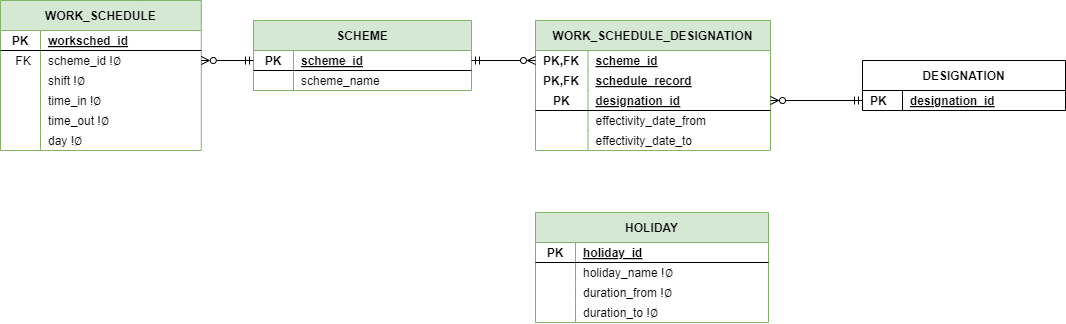
\includegraphics[width=1\linewidth]{figures/images/erd-timesys.png}
        \caption{HRIS TIMESYS ERD Model.}
        \label{fig:erd-timesys}
    \end{figure}

    In this part of the ERD model, it depicts the HRIS TIMESYS, monitoring and recording staff attendance. The system allows for the creation and assignment of various work schedules linked to different schemes and designations. 

    The WORK\_SCHEDULE table captures detailed timing information for each day, crucial for tracking regular attendance. Also, the HOLIDAY table plays a vital role in attendance monitoring by defining non-working days that should not be counted as absences. This distinction is essential for accurate attendance records. The WORK\_SCHEDULE\_DESIGNATION table, with its effectivity dates, enables tracking of schedule changes over time. This structure facilitates flexible management of work schedules while ensuring precise attendance monitoring that correctly accounts for holidays and regular working days across different roles and time periods.

    \begin{figure}[H]
        \centering
        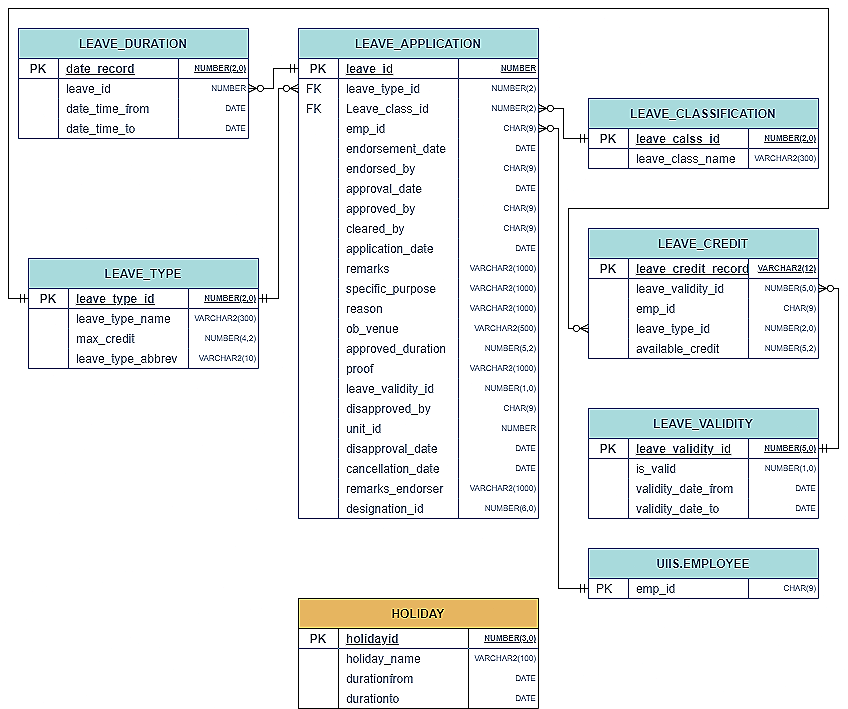
\includegraphics[width=1\linewidth]{figures/images/erd-leavesys.png}
        \caption{HRIS LEAVESYS ERD Model.}
        \label{fig:erd-leavesys}
    \end{figure}

    This section of ERD model depicts a comprehensive HRIS LEAVESYS designed to handle employee leave applications and processing. The diagram centers around the LEAVE\_APPLICATION entity, which connects to various supporting entities such as LEAVE\_TYPE, LEAVE\_CLASSIFICATION, LEAVE\_DURATION, and LEAVE\_VALIDITY. It shows how employee data from UIIS.EMPLOYEE links to leave applications, and how the system manages different types of leave, their classifications, durations, and associated credits. The ERD captures the full lifecycle of a leave request, including submission, endorsement, approval, clearance, and potential cancellation or disapproval. It also incorporates features for tracking leave credits, validity periods, and specific details of each leave application, providing a robust framework for efficient and detailed leave management in an organization.

    \begin{figure}[H]
        \centering
        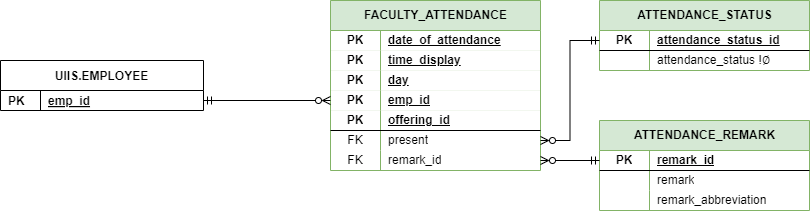
\includegraphics[width=1\linewidth]{figures/images/erd-facsys.png}
        \caption{HRIS FACSYS ERD Model.}
        \begin{description}
            \item[] This segment of the ERD model illustrates the HRIS FACSYS module, which focuses on monitoring and recording faculty attendance. It centers around the FACULTY\_ATTENDANCE entity, which records detailed attendance information, including date, time, day, and associated course offerings for each employee. The system links to a separate UIIS.EMPLOYEE entity, containing broader employee data. It incorporates two supporting entities: ATTENDANCE\_STATUS for categorizing attendance and ATTENDANCE\_REMARK for additional notes. This structure allows for comprehensive tracking of faculty attendance, supporting multiple class offerings per employee and providing flexibility in recording attendance statuses and remarks. The design enables efficient record-keeping and could facilitate various attendance-related analyses and reports.
        \end{description}
        \label{fig:erd-facsys}
    \end{figure}
    
    \subsection{Gantt Chart}
    
    Gantt chart allows for a visual representation of the project schedule that outlines the tasks, milestones, and dependencies throughout the development time. In connection with the development of project management strategy through RAD, the HRIS application's use of a Gantt chart will help in planning and tracking the project's progress. It will break down the development process into specific tasks, assign responsibilities, and establish timelines for each phase of the project.
    
    With this, the development team can effectively manage resources, monitor progress, and ensure that the project stays on track to meet the specified deadlines.

    \begin{figure}[H]
        \centering
        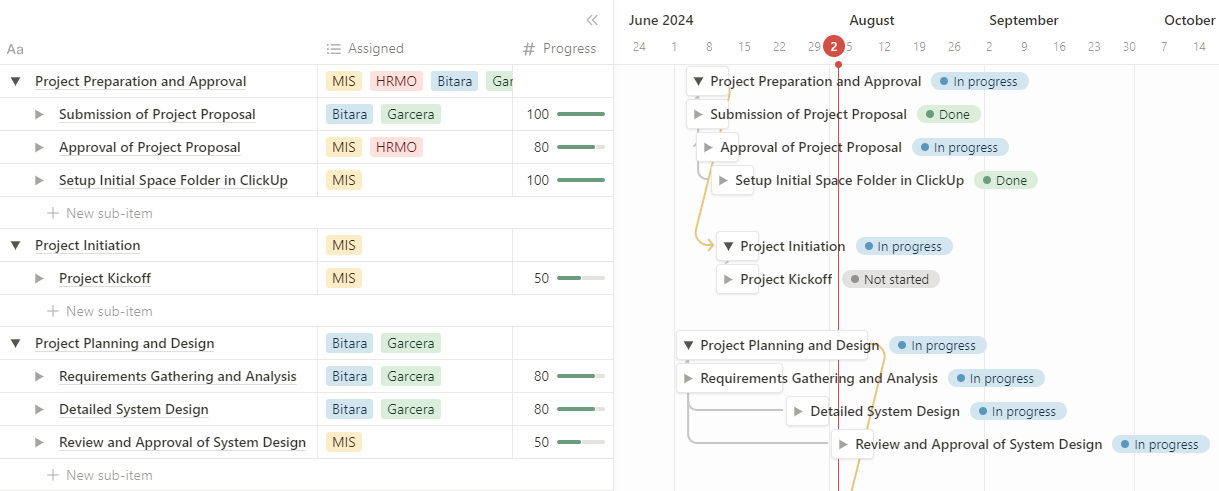
\includegraphics[width=1\linewidth]{figures/images/gantt-chart-1.png}
        \caption{HRIS Gantt Chart Pre-planning Timeline.}
        \label{fig:gantt-chart-1}
    \end{figure}

    The gantt chart in figure \ref{fig:gantt-chart-1} illustrates the pre-planning timeline for the HRIS project. It outlines the key tasks and milestones that need to be completed before the development phase begins. This includes submission and approval of the project proposal, project management setup, to requirements gathering and system design. The timeline provides a clear overview of the project's initial stages and sets the foundation for the subsequent development phases.

    \begin{figure}[H]
        \centering
        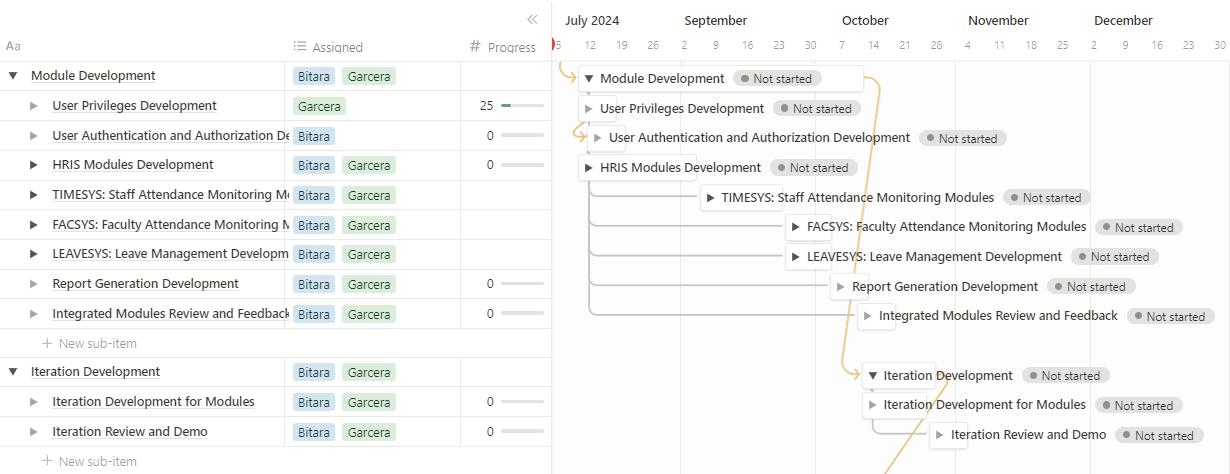
\includegraphics[width=1\linewidth]{figures/images/gantt-chart-2.png}
        \caption{HRIS Gantt Chart Modules Development Timeline.}
        \label{fig:gantt-chart-2}
    \end{figure}

    In the figure \ref{fig:gantt-chart-2}, the gantt chart outlines the timeline for the modules development phase of the project. It breaks down the development process into specific tasks and assigns responsibilities to the development team. The timeline includes tasks from the user authentication to HR core modules, to TIMESYS, LEAVESYS, and FACSYS. During the development phase of the project, the developers shall also make iterations and adjustments based on user feedback and testing results.

    \begin{figure}[H]
        \centering
        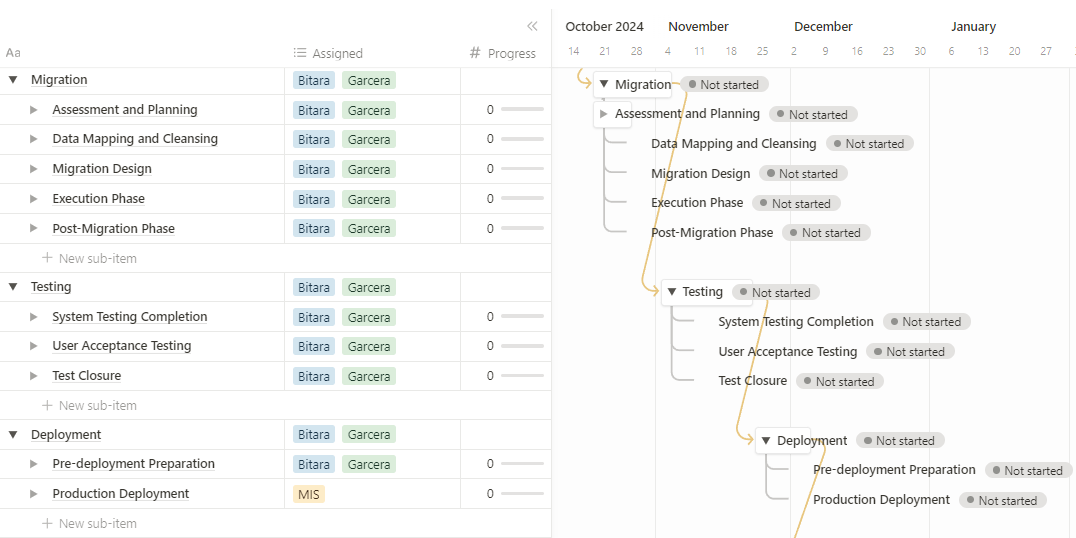
\includegraphics[width=1\linewidth]{figures/images/gantt-chart-3.png}
        \caption{HRIS Gantt Migration to Deployment Timeline.}
        \label{fig:gantt-chart-3}
    \end{figure}

    In the figure \ref{fig:gantt-chart-3}, the gantt chart outlines the timeline for the migration phase of the project. Wherein, it will require other entities such as the HR, ISS, DBA, and MIS to work together to ensure a smooth transition of data from the existing HRIS system to the new HRIS application. The timeline includes migration plan, testing phase, and deployment phase.

    \begin{figure}[H]
        \centering
        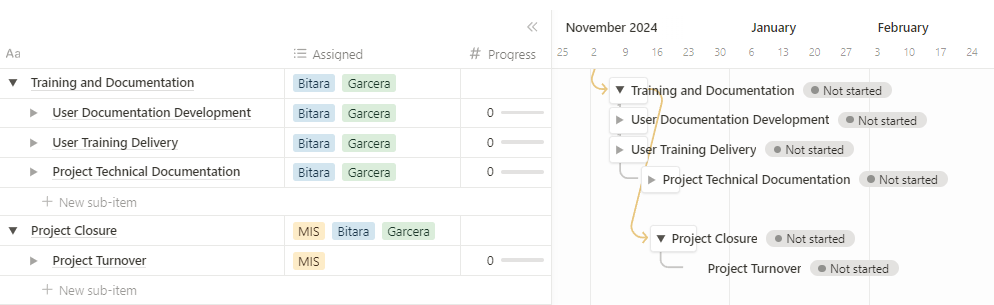
\includegraphics[width=1\linewidth]{figures/images/gantt-chart-4.png}
        \caption{HRIS Gantt Post Development Timeline.}
        \label{fig:gantt-chart-4}
    \end{figure}

    After the deployment phase, the gantt chart in figure \ref{fig:gantt-chart-4} outlines the timeline for the post-development phase of the project. This includes creating trainings and documentations for the HRIS application, providing support, and monitoring the system's performance e.g., user manual, user trainings, and technical documentations. Once accomplished, the project will be handed over to MIS for further management and maintenance.

\section{Data Migration Plan}

    \subsection{Objectives}

    The data migration plan aims to ensure a smooth and efficient transition of data from the existing HRIS system to the new HRIS application. The key objectives of the data migration plan include:

    \begin{enumerate}
        \item Identify and extract relevant data from the existing HRIS system.
        \item Transform and map the data to align with the new HRIS database schema.
        \item Load the data into the new HRIS application while ensuring data integrity and accuracy.
        \item Validate the migrated data to ensure completeness and consistency.
        \item Minimize downtime and disruptions to the HR operation.
        \item Document the data migration process and outcomes for future reference.
    \end{enumerate}

    \subsection{Data Migration Strategy}

    The data migration strategy will involve the following key steps:
    
        \subsubsection{Assessment and Planning}
            This phase invovles identifying the key stakeholders, analyzing the current HRIS that being utilized, gathering requirement for the new system. Having a proper assessment and planning are crucial in understanding the scope of the migration, identifying potential risks, and setting clear objectives. This phase ensures that all stakeholders are aligned and that the migration plan addresses all necessary aspects of the project. Also, effective planning will help mitigate risks and lays a solid foundation for the migration process.

        \subsubsection{Data Mapping and Cleansing}
            In this phase, it includes aligning the data fields from the legacy system to the new HRIS and correcting data quality issues. To ensure that all important data is correctly transferred to the new system, having an proper or accurate data mapping is needed. This phase also includes data cleansing as it is essential for maintaining data integrity and ensuring that the new system operates with accurate and reliable data. This step is critical for preventing data-related issues post-migration and ensuring a smooth transition.

        \subsubsection{Migration Design}
            The Migration design involves selecting migration tools  and deciding on the migration approach. Choosing the necessary and right tools and approach can significantly reduce the risk of errors and downtime. With a well-designed migration process ensures that data is transferred efficiently and securely. This step is important for optimizing the migration process and ensuring that it aligns with the project’s goals and constraints
        
    \subsection{Execution Phase}
        \subsubsection{Pilot Migration}
            Conducting a pilot migration involves setting up a test environment and performing a trial run with a subset of data. A pilot migration helps identify potential issues and validate the migration process before the full migration. Also, with this step it helpful for minimizing risks and ensuring a smooth transition. It allows for adjustments to be made based on the findings from the pilot, thereby improving the overall migration strategy

        \subsubsection{Full Migration}
            In this full migration, it involves extracting, transforming, and loading the full dataset into the new system. Proper execution ensures that all data is accurately transferred and that the new system is ready for use. Validation and reconciliation are essential to confirm data integrity and completeness. This step is the core of the project and requires meticulous planning and execution to ensure success

    \subsection{Post-Migration Phase}
        Post-migration activities include system testing, data validation, user training, and providing support. These activities ensure that the new system operates correctly, that data integrity is maintained, and that users are comfortable with the new system. Ongoing support helps address any issues that arise after the migration. This step is crucial for ensuring the long-term success of the new system and for achieving user satisfaction
    
\section{System Testing Plan}

    The system testing phase aims to comprehensively evaluate the functionality, performance, and reliability of the application. To ensure a thorough assessment, we have established the following key objectives within the system testing plan:
    
    \begin{enumerate}
        \item Verify the functionality of all system features and modules.
        \item Ensure the system meets all specified requirements.
        \item Identify and document any bugs or issues.
        \item Validate the system's performance and response times.
        \item Test the user interface for usability and intuitiveness.
        \item Confirm data integrity and security measures.
        \item Assess the system's compatibility with different browsers and devices.
    \end{enumerate}

    \subsection{Participants}

    Throughout the testing phase, the participants will include the HR managers as well as the Information System Administrator, and the DBA Administrators.

    \subsection{Equipment and Hardware Requirements}

    The requirements for using the application is minimal due to its chosen deployed platform -- web. The application will only require any modern device that can access the internet through modern up-to-date browsers; specifically Google Chrome version 96 and above. 
    
    The testing phase will be conducted within University grounds as it will require the University's internal network for it to be accessed. 

\section{System Deployment Plan}

This section contains some of the high-level tasks and considerations that will be addressed during the deployment phase of the newly developed and migrated ADNU HRIS.

    \subsection{Deployment Planning}
        
        The deployment plan identifies the requirements and responsibilities of both the client and the development team in preparation for deployment. This includes accomplishing HR requirements -- HR core modules, TIMESYS, LEAVESYS, and FACSYS after reaching satisfaction within the testing plan.

    \subsection{Resources}
        \subsubsection{Facilities}

        The facilities required for testing and deployment to the new HRIS will be conducted within the HR office grounds equipped with modern computers as well a reliable and high-speed internet connection.

        \subsubsection{Hardware}

        The hardware required for running the application shall include:

        \begin{enumerate}
            \item Desktop Computers/Laptops
            \begin{enumerate}
                \item \textbf{Processor:} Minimum Intel Core i3 or AMD equivalent
                \item \textbf{RAM:} Minimum of 4GB (recommended 8GB or higher)
                \item \textbf{Storage:} Minimum of 128GB (recommended 256GB or higher)
            \end{enumerate}
            
            \item Backup and Recovery Hardware
            \begin{enumerate}
                \item \textbf{Backup Power supply:} This is to avoid downtime during any power outages to ensure uninterrupted workflow. Ensure that there is a Uninterruptible Power Supply (UPS) systems for critical hardware.
                
                \item \textbf{Electric Generators:} This is to for any extend outages that can occur within operations time. This ensures that the University can still cater and be operational despite the outages.
            \end{enumerate}
            
            \item Peripheral Devices
            \begin{enumerate}
                \item \textbf{DTR Scanner:} The HR module TIMESYS will utilize the DTR Scanner for employee attendance purposes.
                \item \textbf{RFID Scanner:} The RFID scanner will be utilized in support for the DTR within HR.
            \end{enumerate}
            
        \end{enumerate}

        \subsubsection{Support Software}

        As the project will utilize Oracle for the data migration, the supported software shall be to use Oracle 12c with instantclient12 installed and sqldeveloper for the database management solution. 

        Being a web-based application, the project requires to run on modern browsers with version 96 and above for Google Chrome. This ensures better up-to-date features and better security patches for each devices.

        \subsubsection{Support Documentation}

        The documentation required to support the application shall include:

        \begin{itemize}
            \item[] \textbf{User Manuals:} Detailed guides for end-users to navigate and utilize the HRIS effectively.
            \item[] \textbf{Technical Documentation:} In-depth documentation for developers detailing the system architecture, database schema, and configuration settings.
            \item[] \textbf{Training Materials:} Resources for training sessions, including slides, and user manuals.
            \item[] \textbf{FAQs and Troubleshooting Guides:} Common issues and their resolutions to assist users and support staff under user manual.
            \item[] \textbf{System Requirements:} Specifications for hardware, software, and network configurations needed to run the new HRIS.
        \end{itemize}

    \subsection{Deployment Strategies}
    
    The project will be deployed through a series of code review, database review, iteration, and installation of the developed app to the server after a series of testing and acceptance to the application. This process involves multiple personnel including the DB Administrator, Senior Application Developer, and Information System Administrator. 
    
    \subsection{Contingencies}
    
    Contingency plans are ensured to mitigate any potential issues that may arise during and after deployment, the following contingency plans will be put in place:

    \begin{itemize}
        \item[] \textbf{Rollback Plan:} A rollback strategy will be developed and practiced for each implementation to revert to the previous system in case of any critical failures during deployment. This includes utilizing version controls and maintaining a full backup of the old system.

        \item[] \textbf{Performance Monitoring:} Includes continuous monitor of system performance post-deployment through feedback and user reports from the HR for any performance degrade.
    \end{itemize}

    \subsection{Compatibility Strategies}
 
    To ensure smooth deployment and integration of the new ADNU HRIS, the following compatibility strategies will be implemented:
    
    \begin{itemize}
        \item[] \textbf{System Compatibility Testing:} Rigorous testing will be conducted to ensure the new HRIS is compatible with existing hardware, software, and network infrastructure at ADNU.
        
        \item[] \textbf{Browser Compatibility:} The web-based application will be tested across multiple browsers and versions to ensure consistent functionality and appearance.
        
        \item[] \textbf{Integration Testing:} Comprehensive testing will be performed to verify seamless integration with other existing systems and databases at ADNU.
        
        \item[] \textbf{Legacy System Compatibility:} Where necessary, interfaces or middleware will be developed to ensure compatibility with any legacy systems that need to interact with the new HRIS.
        
        \item[] \textbf{Scalability Testing:} The system will be tested to ensure it can handle increased load and user numbers as the university grows. This includes data optimization during any reports or querying. 
    \end{itemize}
    
\section{System Snapshots}

In this section, contains some of the few initial screen mock-ups for redesigning among the major services of the previous HR system. This includes samples high-fidelity wire frame made in Figma. This allows for better visualization to the expected output for the new ADNU HRIS.

    \begin{figure}[H]
        \centering
        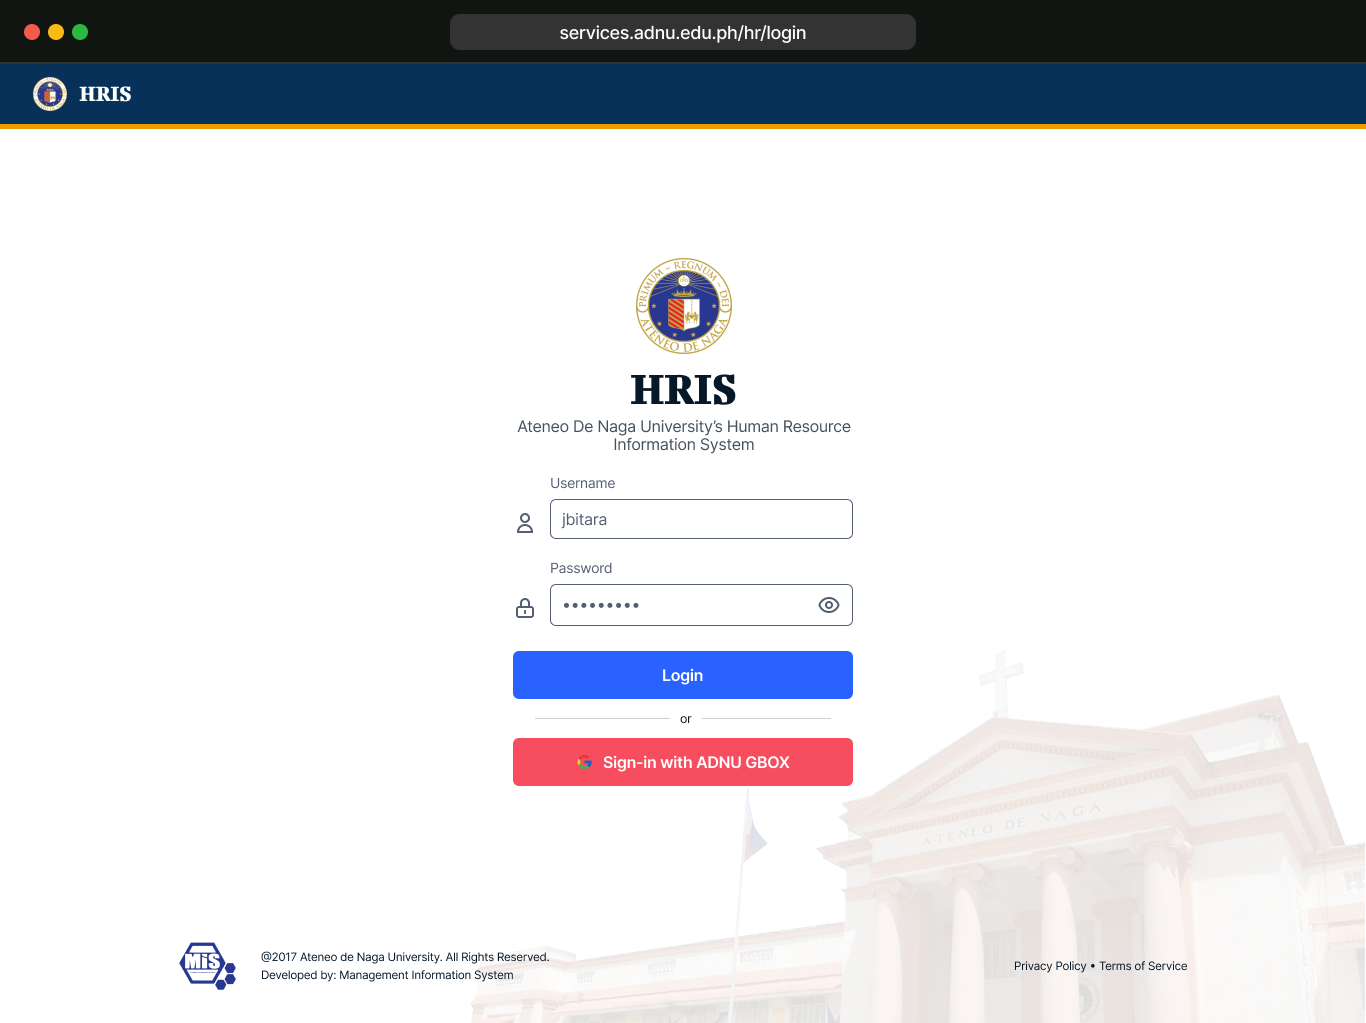
\includegraphics[width=1\linewidth]{figures/app/login.png}
        \caption{New HRIS Login Page.}
        \label{fig:app-login}
    \end{figure}

    The new design displays the redesigned login page. It features a clean, modern interface with input fields for username and password, as well as a prominent login button. The design emphasizes user-friendliness and security for accessing the HRIS platform.

    \begin{figure}[H]
        \centering
        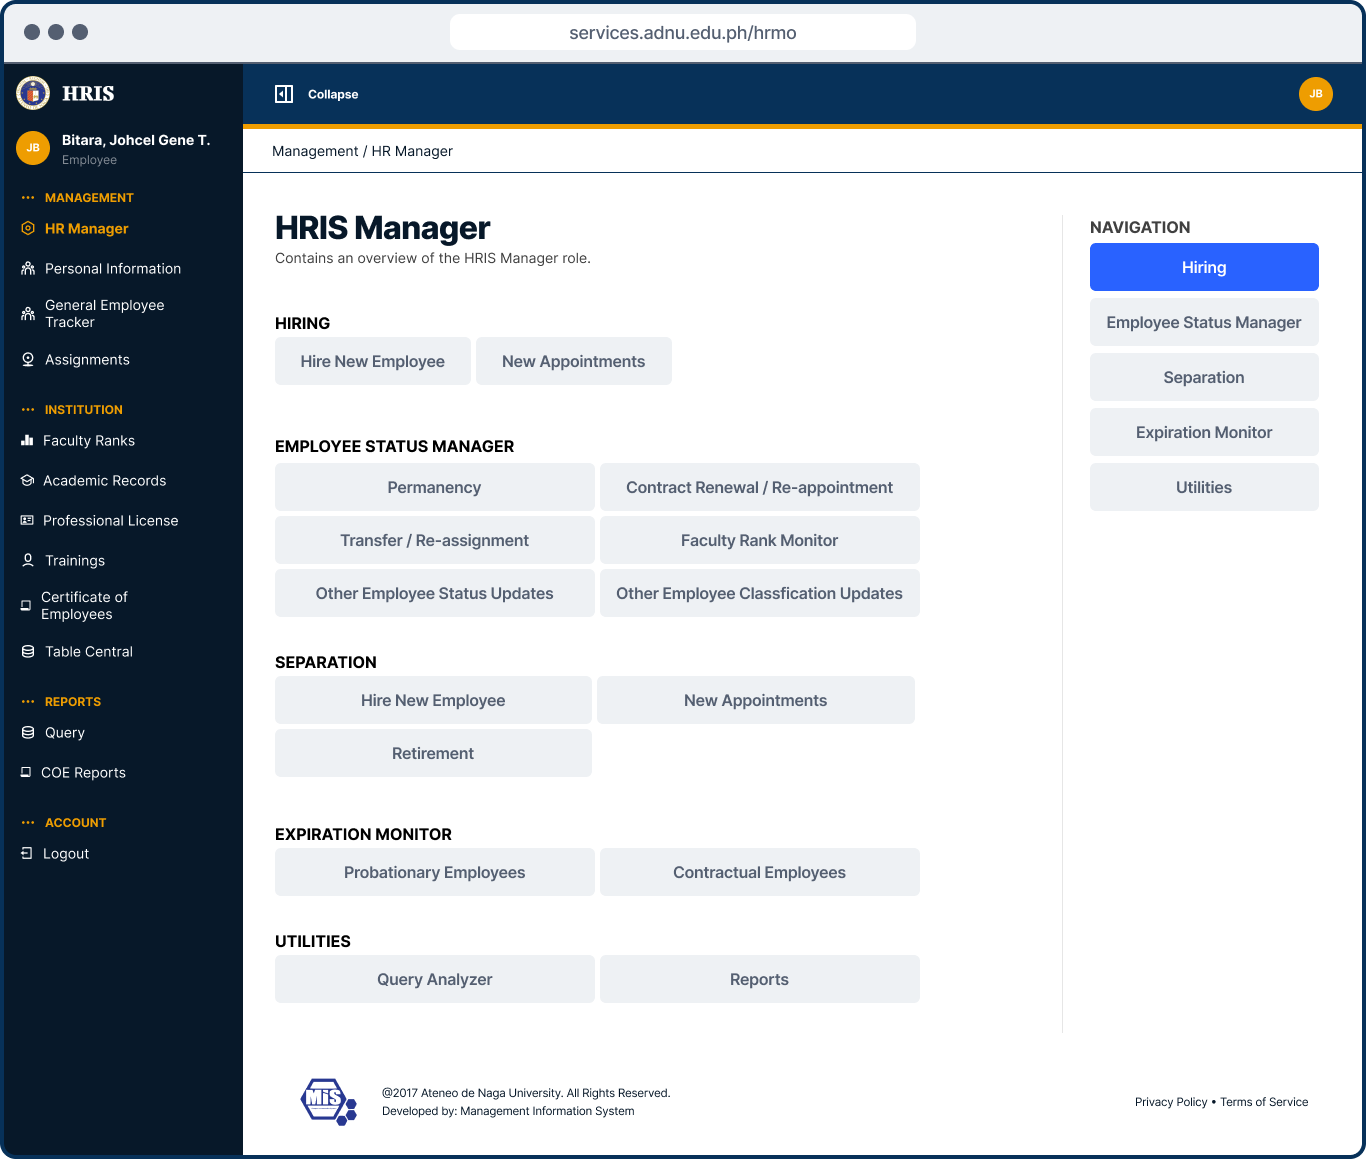
\includegraphics[width=1\linewidth]{figures/app/manager.png}
        \caption{New HRIS Manager Page.}
        \label{fig:app-manager}
    \end{figure}

    The figure presents the newly designed HRIS Manager page. This includes mainly making use of better user experience with enlarged buttons and easier navigation with the use of better UI layout.

    \begin{figure}[H]
        \centering
        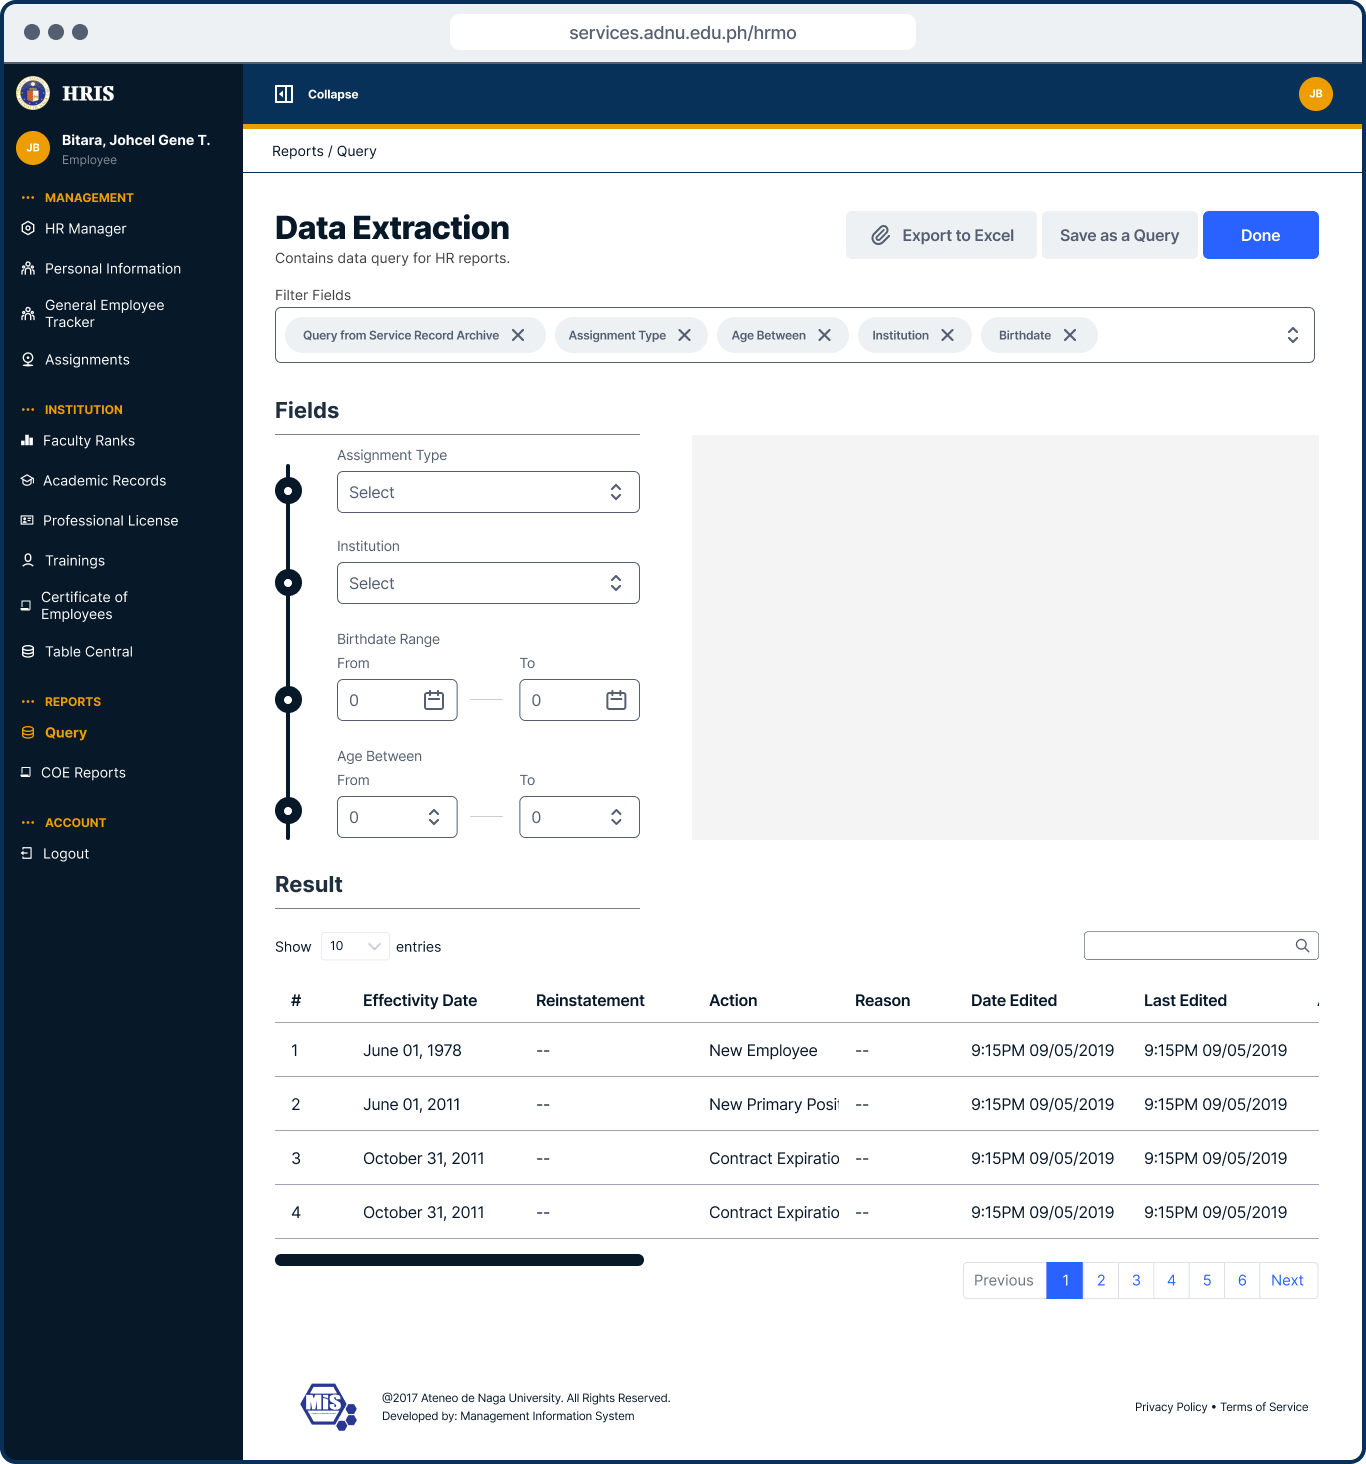
\includegraphics[width=1\linewidth]{figures/app/data-extraction.png}
        \caption{New HRIS Data Extraction Page.}
        \label{fig:app-data-extraction}
    \end{figure}

    This figure showcases the new Data Extraction Page. The interface is designed to facilitate efficient retrieval of HR data, likely offering options for customizable reports, data filtering, and export functionalities.

    \begin{figure}[H]
        \centering
        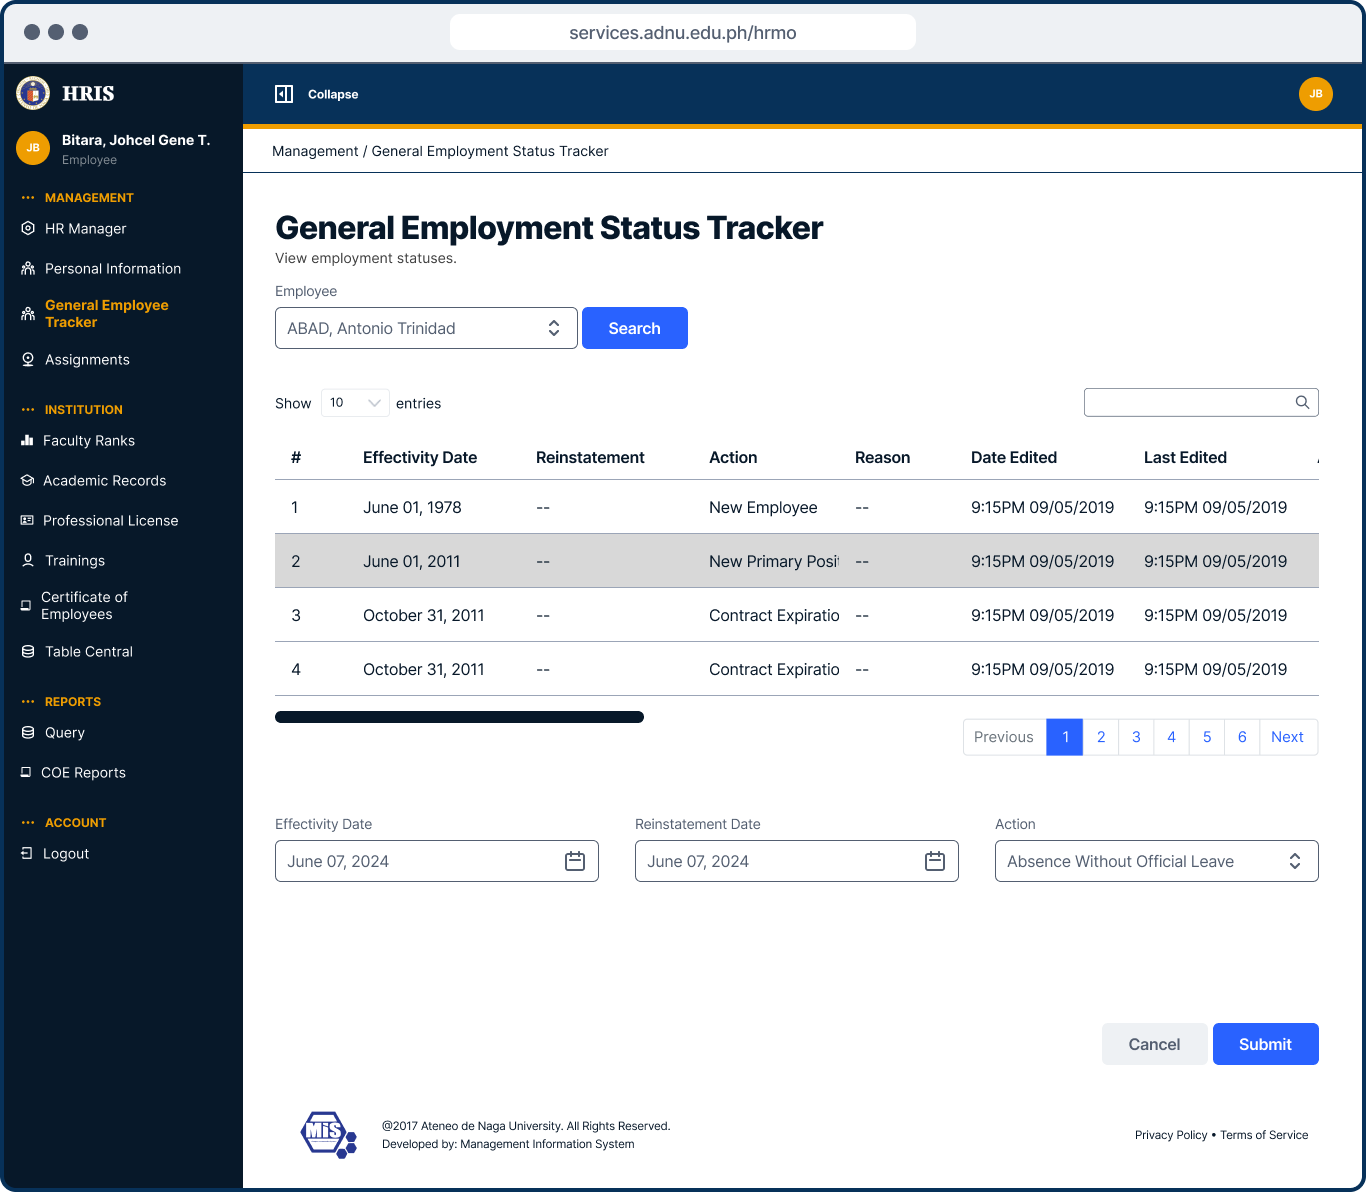
\includegraphics[width=1\linewidth]{figures/app/gest.png}
        \caption{New General Employment Status Tracker Page.}
        \label{fig:app-gest}
    \end{figure}

    This figure illustrates the new General Employment Status Tracker (GEST) page. The GEST interface likely provides a comprehensive view of employee statuses across the organization. It includes employment types, contract durations, leave statuses, and other key indicators of workforce composition. 

    \begin{figure}[H]
        \centering
        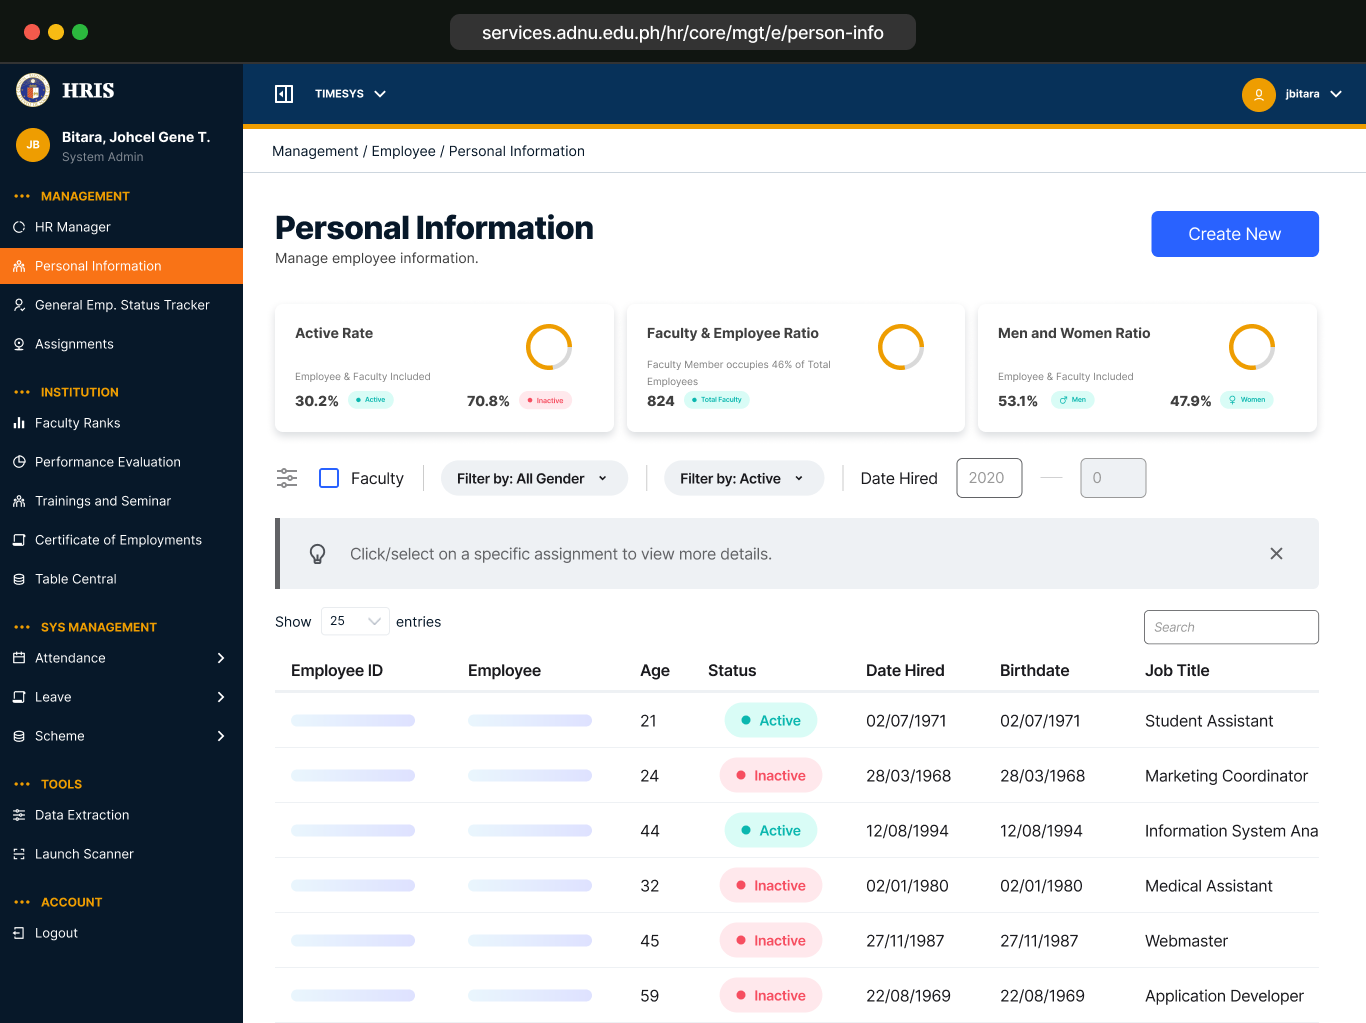
\includegraphics[width=1\linewidth]{figures/app/pi.png}
        \caption{Personal Information for All Employees.}
        \label{fig:app-pi}
    \end{figure}

    This figure displays all the basic personal information for all employees in table view. This includes their personal information. Admins can select among the employees to view more of their personal information.

    \begin{figure}[H]
        \centering
        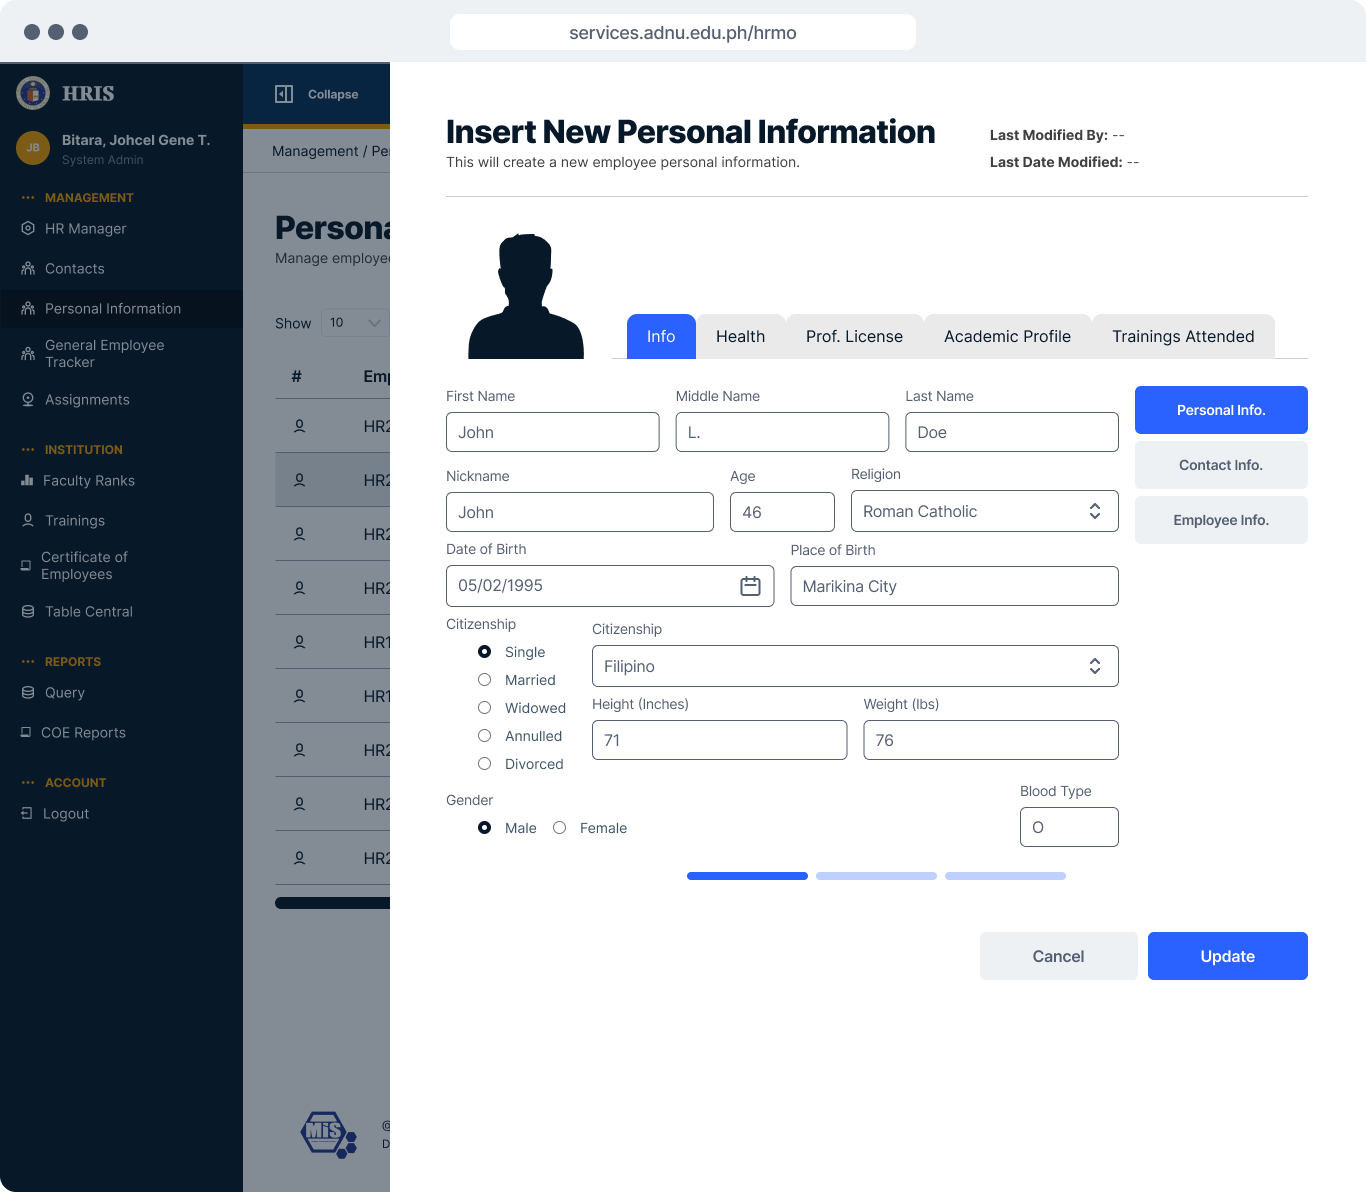
\includegraphics[width=1\linewidth]{figures/app/pi-insert.png}
        \caption{Creating New Personal Information in the Record.}
        \label{fig:app-pi-insert}
    \end{figure}

    This figure displays the interface for creating new personal information in the record. Admins can input the necessary information for the employee to be added to the system.

    \begin{figure}[H]
        \centering
        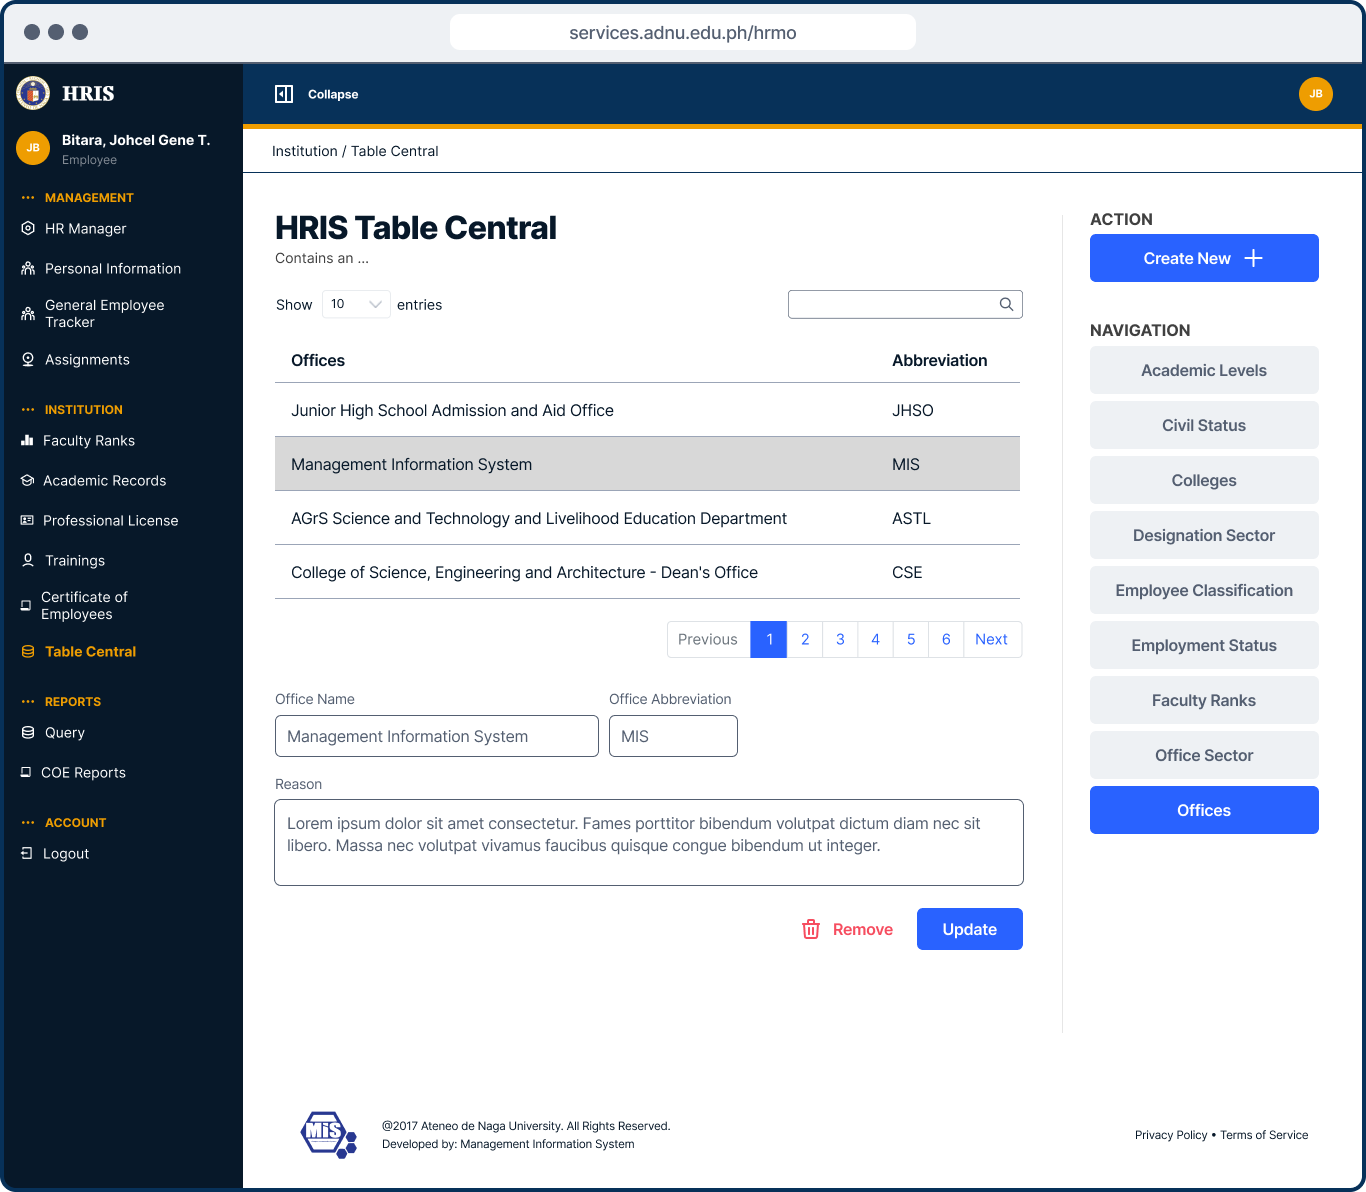
\includegraphics[width=1\linewidth]{figures/app/table-central.png}
        \caption{New HRIS Table Central Page.}
        \label{fig:app-table-central}
    \end{figure}

    This figure displays the HRIS Table Central module wherein, managers can manage certain sectors and department information and make updates within the University.

    \begin{figure}[H]
        \centering
        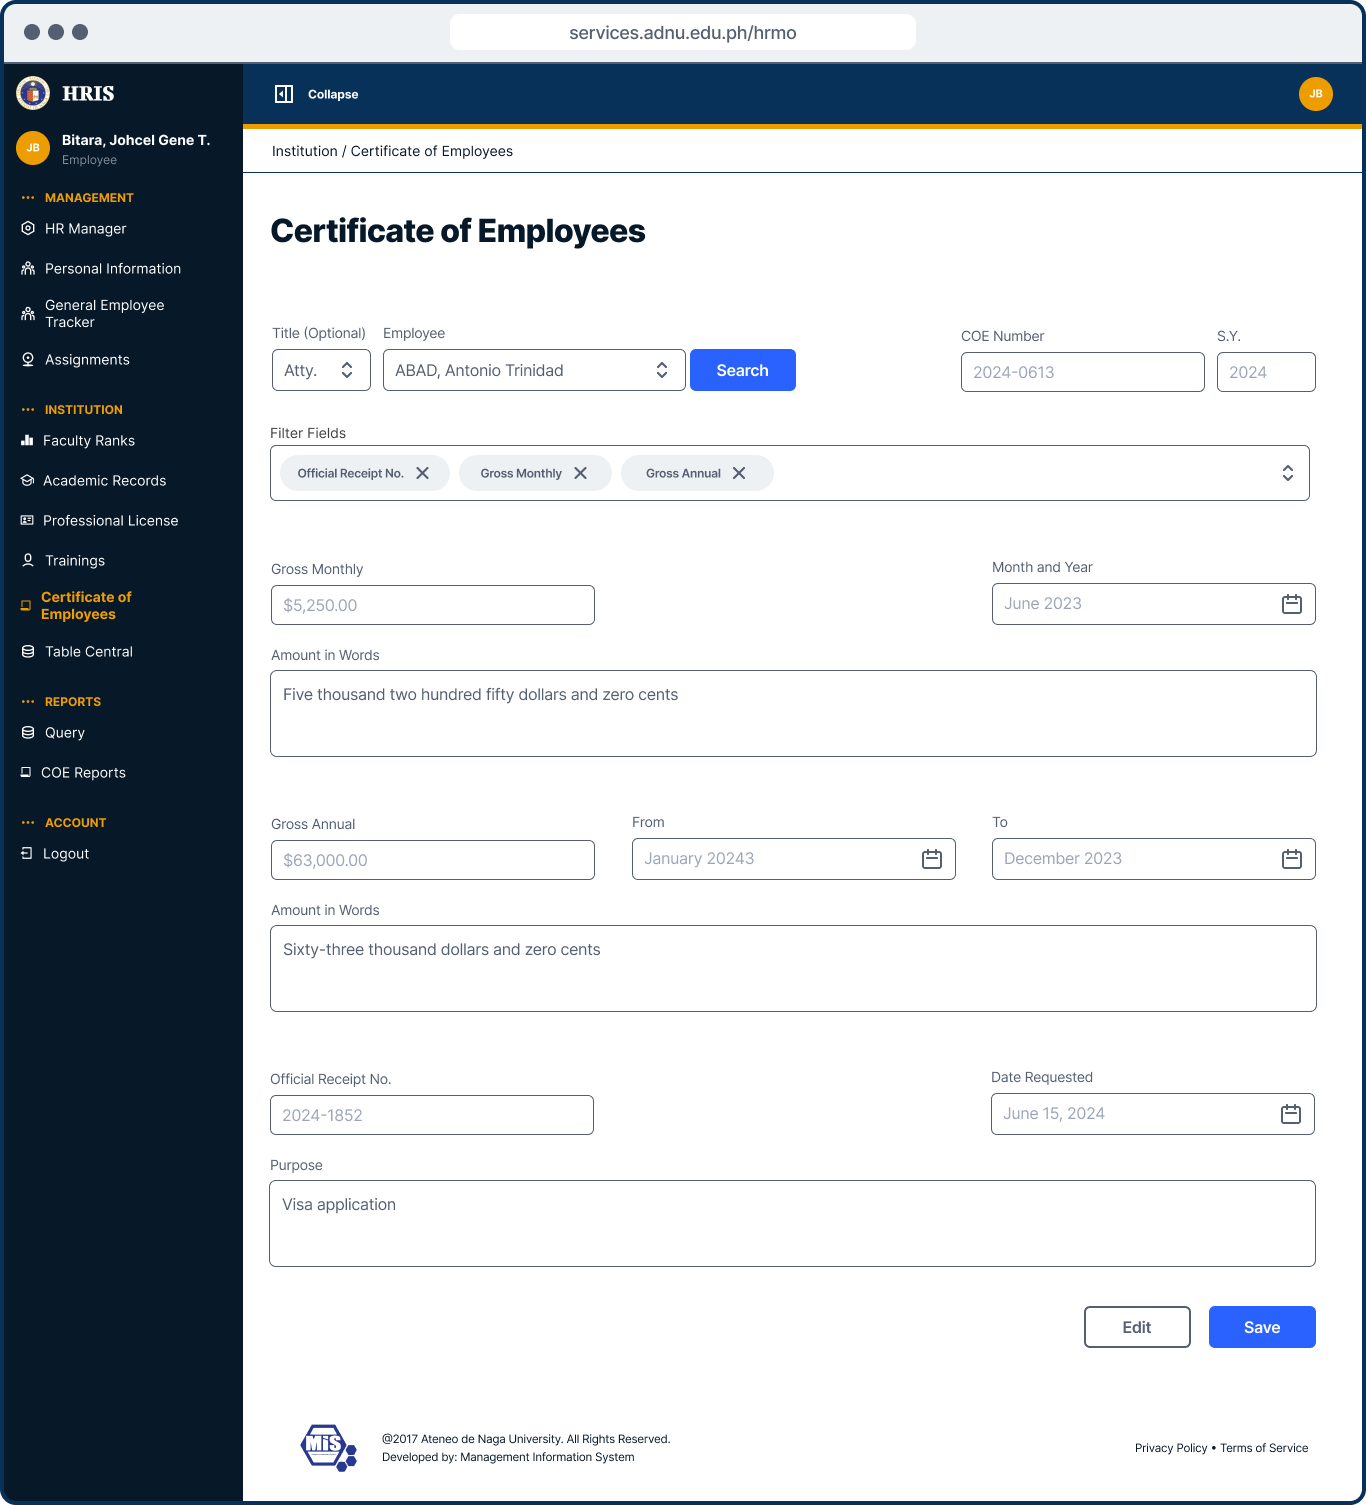
\includegraphics[width=1\linewidth]{figures/app/coe.png}
        \caption{New HRIS Certificate of Employment Processing Page.}
        \label{fig:app-coe}
    \end{figure}

    This interface is designed to streamline the creation and issuance of employment certificates. Managers can select employees and generate COE for each University personnel.